\documentclass[12pt]{article}
\usepackage[utf8]{inputenc}
%\usepackage{csquotes}
\usepackage{graphicx}
\graphicspath{ {pictures/} }
\usepackage{caption}
\usepackage{subcaption}
\usepackage[a4paper,width=150mm,top=25mm,bottom=25mm,bindingoffset=6mm]{geometry}
\usepackage[english]{babel}
\usepackage{amsthm,etoolbox, amsmath, amssymb}
\DeclareMathOperator*{\argmax}{arg\,max}
\DeclareMathOperator*{\argmin}{arg\,min}
\usepackage{enumitem}   
\usepackage[nottoc]{tocbibind}
\usepackage{hyperref}
\usepackage[nameinlink, capitalise, noabbrev]{cleveref}
\usepackage{wrapfig}
\usepackage{color} 
\usepackage [autostyle, german = quotes]{csquotes}
\usepackage{tikz}
\usepackage{pgffor}
\usepackage{listings}
\usepackage{fancyhdr}
\usepackage{setspace}
\usepackage{algorithm}
\usepackage{algpseudocode}
\usepackage{multirow}
\usepackage{tikz}
\usepackage{circuitikz}
\usetikzlibrary{positioning, arrows.meta, shapes, calc, fit}
\graphicspath{ {../images/} } 
\setstretch{1.33}
\MakeOuterQuote{"}

\AddToHook{cmd/section/before}{\clearpage}

\theoremstyle{plain}
\newtheorem{thm}{Theorem}
\newtheorem{lem}[thm]{Lemma}
\newtheorem{prop}[thm]{Proposition}
\newtheorem{cor}[thm]{Corollary}

\theoremstyle{definition}
\newtheorem{definition}[thm]{Definition}
\newtheorem{ex}[thm]{Example}
% \AtBeginEnvironment{ex}{
%   \pushQED{\qed}\renewcommand{\qedsymbol}{\par\noindent\rule{0.33\textwidth}{0.2pt}}
% }
% \AtEndEnvironment{ex}{\popQED\endexample}
\theoremstyle{remark}
\newtheorem{rem}[thm]{Remark}

\makeatletter
\@addtoreset{thm}{section}% Reset theorem counter with every section
\@addtoreset{thm}{subsection}
\@addtoreset{thm}{subsubsection}
\newcommand{\theoremprefix}{}
\let\thetheoremsaved\thethm
\renewcommand{\thethm}{\theoremprefix\thetheoremsaved}
\let\sectionsaved\section
\patchcmd{\@startsection}{\par}{\renewcommand{\theoremprefix}{\csname the#1\endcsname.}}{}{}
\makeatother

\setlength{\jot}{10pt}
\setlength{\headheight}{15pt}

\newcommand*\circled[1]{\tikz[baseline=(char.base)]{%
            \node[shape=circle,fill=blue!20,draw,inner sep=2pt] (char) {#1};}}

\usepackage[style=alphabetic, firstinits=true, backend=biber, sorting=nyt, doi=false, isbn=false, url=true, maxbibnames=99]{biblatex}
\DeclareNameAlias{default}{family-given}
\addbibresource{references.bib}

\title{Thesis Title}
\author{Author Name}
\date{Day Month Year}

\setlength\parindent{0pt}

\begin{document}
	\pagenumbering{gobble}
	\begin{titlepage}
	\begin{center}
		\vspace*{1cm}
		
\includegraphics{TU_Logo_kurz_1c_schwarz.eps}\\
		\Large
		Technische Universität Berlin\\
		Institut für Mathematik
		\vspace*{1cm}



		\Huge
		\textbf{Numerischer Wertebereich}
		
		\vspace{0.5cm}
		\LARGE
		und Anwendung auf das Lax-Wendroff-Verfahren
		
		\vspace{1.5cm}
		
		\textbf{Sijun John Tu}
		
		\vfill
		
		Bachelorarbeit \\
		zur Erlangung des Grades\\
		Bachelor of Science \\
		im Fach Mathematik
		
		\vspace{0.8cm}

		
		
		Betreuerin: Frau Dr. Agnes Radl\\
		Zweitgutachterin: Prof. Dr. Tanja Eisner \\
		
	\end{center}
\end{titlepage}
	
\subsubsection*{Abstract}

    In this paper, we investigate the so-called numerical value range of a linear, bounded operator in a Hilbert space. Similar to the spectrum of an operator, the numerical range of values helps to determine certain properties of the corresponding operator to be investigated. In doing so, we will often encounter relations between there two invariants. The main objective of this section is the so-called Power Inequality, a statement about the numerical radius of powers of an operator, as well as the norm property of the numerical radius. In particular, an algorithm is presented and implemented, which numerically approximates the numerical value for a finite-dimensional operator. In the final chapter of the thesis, an application of the numerical value range in numerical mathematics is considered.


	\thispagestyle{empty}
\section*{Eidesstattliche Erklärung}

Hiermit erkläre ich, dass ich die vorliegende Arbeit selbstständig und eigenhändig sowie ohne unerlaubte fremde Hilfe und ausschließlich unter Verwendung der aufgeführten Quellen und Hilfsmittel angefertigt habe.\\

Die selbstständige und eigenhändige Anfertigung versichert an Eides statt:\\\\\\\\\\
Berlin, den \today \\[5cm]
\rule{10cm}{0.4pt}\\
Sijun John Tu
	\thispagestyle{empty}
\section*{ACKNOWLEDGEMENT}

This thesis was carried out at RISE Cybersecurity unit as part of KTH's Master's programme in Applied anc Computational Mathematics. I would like to express my gratitude towards my supervisors Shahid Raza, Anders Szepessy and Alfonso Iacovazzi for making this project possible. Furthermore, I would like to thank Apostolos Pyrgelis and Han Wang for their unwavering support and expertise.\\
\\[2cm]

Sincerely,
\\[1cm]

Sijun John Tu

Stockholm, \today


	\tableofcontents
	
	\clearpage
	\pagenumbering{roman}
	\setcounter{page}{1}
	
\section*{Notation}
Mathematical conventions and notation used in this thesis:

\begin{center}
    \renewcommand{\arraystretch}{1.5}
    \begin{tabular}{ c l }
        
        $\mathbb{R}$ & the real numbers \\
        $\sqcup$ & disjoint set union \\
        $\mathcal{N}(\mu, \sigma^2)$ & Gaussian distribution with mean $\mu$ and variance $\sigma^2$
    \end{tabular}
\end{center}

Additionally, we introduce the following conventions to describe various elements from different mathematical objects to make the notations and their meaning as consistent as possible:

\begin{center}
    \renewcommand{\arraystretch}{1.5}
    \begin{tabular}{c l}
        $\mathcal{S}$ & set of heartbeat samples \\
        $s_i \in \mathbb{R}^L$ & seqeunce of ECG measurements \\
        $\mathcal{K}^X$ & arrhythmia detection model trained on some training data $X$


    \end{tabular}
\end{center}

	\addcontentsline{toc}{section}{Notation}

	\clearpage
	%\listoffigures
	{
	\let\oldnumberline\numberline
	\renewcommand{\numberline}{\figurename~\oldnumberline}
	\listoffigures
	}
	\clearpage
	\pagestyle{fancy}
	\fancyhf{}
	\fancyhead[L]{\leftmark}
	\fancyfoot[R]{\thepage}

	\pagenumbering{arabic}
	\setcounter{page}{1}
	\section{Introduction}

\subsection{Motivation}

Data-driven technology and especially machine learning have gained a lot of momentum the past years. Models like ChatGPT or BERT heavily depend on large datasets that are available publicly. At the same time machine learning models are now being considered in other data sensitive domains like health care \parencite[see][]{ai_and_med,aimed2,aimed3,aimed4}. One exciting field within health care is arrhythmia detection for heartbeats, where machine learning methods can aid physicians to detect irregular heartbeat conditions. Recently, several methods have been proposed, ranging from SVMs to neural networks \parencite[see review][]{arr_rev}.assessed

\paragraph{}
When working with those sensitive data, privacy plays a major role in general acceptance of those models. In some circumstances neural networks can memorise specific data samples, which constitutes a heavy privacy breach \Parencite[see][]{feldman2021does}. For example in \Parencite{carlini19}, Carlini et al.\ recovered credit card numbers from text completion models used by Google. Now governmental institutions like the European Union have established a right to privacy manifested in the General Data Protection Regulation laws\footnote[1]{see https://gdpr-info.eu/}. Previous simple anonymisation attempts that simply removed some identifying attributes (e.\ g.\ name, birthday etc.) have been proven to be ineffective. For example, user profiles from the anonymised dataset used in the infamous Netflix prize have been reconstructed with the help of publicly available data from IMDB~\cite{4531148}. This is why technological advances in the area of privacy-preserving machine learning have increased in the past few years, with the development of various machine learning models that aim to preserve the privacy of individual data records. Protecting privacy becomes crucial for heartbeat data because it can be used to identify patients, thus heavily impacting the patient's privacy \parencite[see heartbeat biometrics][]{heartb_auth,hegde2011heartbeat}.

\paragraph{}
One promising solution \parencite[see][]{jordon2022synthetic} is to replace the original, possibly sensitive data set with a synthetic data set that resembles the original raw data in some statistical properties. Much research has been done to generate tabular or image data, whereas dedicated time series data generation is still a \textit{``burgeoning''} area of research according to a recent benchmark \parencite[][]{ang2023tsgbench}. Regardless of the data type, data generators with no formal privacy guarantees have been shown to still be susceptible to privacy leaks~\cite{stadler2022synthetic}. 

To improve privacy, this thesis aims to analyse the combination of synthetic data with tools from so-called differential privacy. Differential privacy has been developed by Dwork et al \parencite{dwork2006differential} and is widely considered as the mathematical framework to rigorously provide privacy guarantees to privacy-preserving algorithms, relying on applied probability theory and statistics. This thesis will study existing architectures based on private generative AI models, as well as explore the possibility of new solution. Experiments were conducted to assess the performance of these models using the MITBIH dataset on heartbeat arrhythmia \parencite[][]{moody2001impact}. Unfortunately, there is no free lunch and privacy always comes with a decrease in utility~\cite{stadler2022synthetic}. A careful balance between privacy and utility needs to be established. However, we will challenge this trade-off and show that privacy and utility in the use case of anomaly detection can go hand in hand, because it can add some robustness to the model. This was first explored in \Parencite{du2019robust} for detecting anomalies.


\subsection{Problem Definition}

This thesis aims to examine how to generate private time series data for heartbeat arrhythmia detection. Let $\mathcal{S}={\{s_i\}}_{i=1}^N$ denote a set of heartbeat samples, where $s_i=(s_i^0,..., s_i^L)$ is a sequence of one-dimensional ECG measurements of fixed length $L$ corresponding to one heartbeat. Each heartbeat sequence is associated with a corresponding label denoting whether it is a normal or anomalous heartbeat according to ???. Therefore we separate the set into normal heartbeats $\mathcal{N}$ and $\mathcal{A}$ (i.\ e.\ $\mathcal{S} = \mathcal{N} \sqcup \mathcal{A}$)

\paragraph{}

Firstly, we want to design a time series generator (TSG) that can model the true probability distribution $p(\mathcal{N})$ of the normal heartbeats. Here, we only consider normal heartbeats since for the subsequent task of arrhythmia detection we will follow an anomaly detection approach explained next. The aim of the TSG is to generate a synthetic data set $\widehat{\mathcal{N}}$ with distribution $p(\widehat{\mathcal{N}})$ that is ``close'' to the original data $p(\mathcal{N})$.

Secondly, the utility of the generated data is assessed in the downstream task of detecting anomalous heartbeats (heartbeat arrhythmia detection). We treat this task as an anomaly detection task based on reconstruction error ??REF, i.\ e.\ we want to train a model only on normal heartbeats that can reconstruct those samples with low error, but give high reconstruction error when inputting an anomalous sample. Alternatively, one could treat this as a binary classification task, that classifies a given heartbeat sample as either normal or anomalous. Since the ratio of those two classes are heavily imbalanced due to the nature of arrhythmias, we will favour the first approach ??REF.

Lastly, we will embed the generation procedure in a differential privacy setting. This will provide a theoretical framework to assess privacy.

\subsection{Related Works and State of the Art}

\subsubsection*{Privacy in machine learning}
A lot of past efforts have been put into improving the performance of machine learning methods, where the privacy aspect has been neglected. Due to the increased awareness about private individual data and policies like EU's GDPR laws, big tech companies like Apple, Google and even the US Census have been implementing privacy measurements in the their data collection \parencite[see][]{dwork2019differential,abowd2019census}. One of the first groundbreaking works on actually quantifying the privacy leakage in machine learning models has been studied in \parencite{shokri2017membership}, where Shokri et.\ al.\ have designed a framework to perform membership inference attacks (MIA) on basic classification tasks. MIA on machine learning models try to infer whether a certain record has been used when training the respective model. This becomes a privacy issue when e.\ g.\ an adversary can infer whether a certain patient's data was used to train a model associated with a disease. Then the adversary can conclude that this particular patient likely has this disease \parencite[cf.][p. 5]{shokri2017membership}. Hence, their results indicate a strong vulnerability in terms of privacy for data-based models.


Several notions of privacy have been proposed in the last decade, among which Differential Privacy (DP) has emerged as the \textit{``de-facto standard in data privacy''} \parencite{kim2021survey}. Reasons for its popularity according to a recent survey \parencite{surv_dp2021} are among others:

\begin{enumerate}
    \item DP is future-proof and requires no extra knowledge about the adversary.
    \item DP provides rigorous privacy guarantees.
    \item DP provides a notion of privacy budget, which can be adapted to the specific use case to balance privacy and utility.
\end{enumerate}

We will revisit the definition and most important results in Chapter \ref{ch2} of this thesis. The basic idea is to add calibrated, random noise either the data or during model training. Broadly speaking, differential private noise can be injected in three different stages of the modelling pipeline: input, hidden or output layer \parencite[cf.][]{zhao2019differential}. 

???IMGAE ACC TO \parencite{wang2023differential}

Applying some DP mechanism at the input stage can be seen as preprocessing step to either hide sensitive attributes in the data or generating new synthetic dataset. Some earlier works include random perturbation methods described for instance in \parencite{input_levelDP,erm_dp_input}. According to \parencite{wang2023differential} this approach is not utilised frequently because extra prior knowledge about the subsequent task is required to calibrate the right amount of noise. More recent methods focus exclusively on generating data samples by deep learning methods, that in turn employ a DP mechanism at gradient or output level. This will be the focus of the next chapter and hence not be discussed here.

Adding privacy in the hidden layer is sometimes referred to as gradient-level DP. Due to the iterative nature of most training algorithms, extra care needs to be taken to track the privacy loss caused by each iteration. Most notably there is a differential private version of stochastic gradient descent (SGD) called DP-SGD developed by Abadi et al \parencite{Abadi_2016} where the authors have designed a mechanism to track the privacy loss incurred while training. Differential privacy is achieved by clipping the gradient and then adding gaussian noise to the gradient. The clipping step is necessary to ensure that the gradient is bounded. Based on a more relaxed definition of DP, the authors in \parencite{bu2020deep} propose an improved version of DP-SGD called NoisySGD. 

At the output level there are several ways to implement DP. One highly cited approach called the ``Functional Mechanism'' followed by the authors in \parencite{zhang2012functional} perturbs the objective function, so it is independent of the number of training steps. A further refinement of this approach was researched in \parencite{adlm2017}, where Phan et al. developed an algorithm that puts adaptive noise on the features based on its contribution to the output.

Other interesting approaches to incorporating differential privacy into deep learning include the PATE learning method by Papernot et al. \parencite{papernot2017semisupervised}. The idea behind this model is to train ``teacher models'' that will not be published, which in turn are used in a random manner to then train private ``student'' models. 

In a distributed setting approaches like federated learning \parencite{konečný2015federated,Mo2019EfficientAP} have been proposed. Their privacy further analysed in \parencite{mcmahan2018learning} for learning language models.

\vspace*{1em}
For a more in-depth review see e. g. \parencite{surrve_ppml,surv_ppml_2,wang2023differential}


\subsubsection*{Data generation and Privacy}

As we have mentioned earlier, ensuring privacy in machine learning applications is crucial when working with sensitive data. One might naively assume, that synthetic data without any formal privacy guarantees provides enough privacy already by design, but this unfortunately is not the case. Especially when generating with GAN-based networks, recent works have shown that although under some circumstances GANs can satisfy a weak notion of DP, but with a very high $\epsilon$ which corresponds to a very weak privacy guarantee \parencite{lin2021privacy,stadler2022synthetic,jordon2022synthetic}. Combining generative algorithms with DP however is a promising solution to mitigate the privacy issue \parencite{bellovin2019privacy} which will be the focus of this thesis.

While we have outlined several techniques from the state of the art to ensure privacy, most of the methods are tailored for a specific model architecture or use case. On the other hand, synthetic data that has been generated with privacy guarantees can be used in any downstream task without privacy breach. To this end, several deep learning based architectures have been proposed. Following \parencite{hu2023sok}, one can broadly categorise them as follows:
\begin{itemize}
    \item GAN-based
    \item Feature-based
    \item Autoencoder based {\tiny \Parencite[see e. g.][for a generator based on a variational autoencoder that is trained with DP-SGD]{vae}}
    \item Optimal transport based {\tiny \Parencite[see e. g.][for generator based on the so-called Sinkhorn divergence]{cao2021dont}}
    \item Stochastic simulation based {\tiny \Parencite[see e. g.][for a differentially-private diffusion model]{dpgen}}
\end{itemize}

We will present the first two approaches in more detail in chapter \ref{chapter3}.

\subsubsection*{Heartbeat arrhythmia detection}
For the experiments conducted in this thesis we will use the common benchmark data set for heartbeat arrhythmia MIT-BIH \parencite{moody2001impact}. It contains one-dimensional ECG measurements of 47 patients each lasting about 30 minutes. This kind of data is commonly referred to as time series data which due to its time dependency needs to be treated differently than tabular data. Each heartbeat is labelled as one of 16 heartbeat classes by experts. We will follow AAMI ???REF standard to divide those classes into normal and anomalous heartbeats. Finding anomalous heartbeats, i. e. arrhythmia detection, can be linked to several common tasks found in machine learning. For example, one can view this problem as a binary classification problem, where one wishes to train a classifier, that given a heartbeat will classify this as either normal or anomalous. Since this requires a balanced dataset, we follow a different approach from anomaly detection. In particular, we will train a baseline model for arrhythmia detection based on so-called the reconstruction error \parencite[see][for an in-depth survey on anomaly detection with times series]{schmidl2022anomaly}. This is a semi-supervised approach where a model is only trained on normal data. The model learns to encode and reconstruct normal data from a (lower-dimensional) latent space with low reconstruction error, whereas it will reconstruct anomalous data with a higher reconstruction error. This method will also be more useful in real-life applications since 1) heartbeat arrhythmias are rather scarce and 2) there is a lot of heartbeat data being collected but not labelled.

Some efforts have been taken to generate ECG data. Most of the recent approaches deploy a GAN based model to generate heartbeat data \Parencite[see e. g.][]{zhu2019electrocardiogram,Delaney2019SynthesisOR,wang2020accurate} getting favourable results. We will also follow a GAN based approach to generate synthetic ECG data. A very recent paper achieved even better result using a transformer architecture \Parencite[see][]{Kaleli2023GenerationOS}.  

	
	\section{Theoretical background on Differential Privacy}\label{ch2}

In this chapter we briefly describe and derive the most important results from Cynthia Dwork's work on differential privacy that was first introduced in 2006 \parencite{dwork2006differential}. This summary heavily relies on her writings in \parencite{dwork2019differential} as well as lecture notes from \parencite{lecture_CSE711}.

\subsection{Defining differential privacy}
Differential privacy (DP) should be understood as an agreement between the data holder and the data subject: the latter should not be "affected, adversely or otherwise, by allowing [her] data to be used in any study or analysis, no matter what other studies, data sets or information sources are available". This addresses the paradox of learning something useful about a population while learning nothing about the individuals


\begin{ex}[Randomised response]
    In 1965 Warner \parencite{stan65rr} proposes the following random answering procedure: In a study where participants are asked to answer with ``Yes'' or ``No'' whether they have engaged in an illegal or embarrassing activity $A$, they should:
    \begin{enumerate}
        \item Flip a coin
        \item If the coin shows tails, then the participant should respond truthfully.
        \item If the coin shows head, then the participant should flip the coin a second time and answer "Yes" if the second coin shows head and "no" otherwise.
    \end{enumerate}
    This procedure ensures participants' privacy by ``plausible deniability''; each participant's answer has non-zero probability of being truthful or not. By understanding the probabilities of the noise generation process, the data analyst can estimate the true number of ``yes'' and ``no'' answers. To this end, let $p$ be the true percentage of ``yes'' answers, $N$ the total number of participants, $n_{true}$ the true number of ``yes'' responses and $\hat{n}_{obs}$ the observed number of ``yes'' responses. We assume a fair coin with equal probability of showing heads or tails. Then the expected number of ``yes'' answers after applying the described procedure is:
    \begin{align}
        \mathbb{E}(``Yes'') = \frac{1}{4} n_{true} + \frac{1}{4} (N-n_{true}) + \frac{1}{2} n_{true} = \frac{1}{4} N + \frac{n_{true}}{2}
    \end{align}
    We can estimate this using the $\hat{n}_{obs} \approx \mathbb{E}("Yes") = \frac{1}{4} N + \frac{n_{true}}{2}$ and finally solving for $n_{true}$ yields the estimate:
    \begin{align}
        \hat{n_{true}} = 2 \hat{n}_{obs} - \frac{1}{2} N
    \end{align}
\end{ex}


\begin{definition}[Probability Simplex]
    Given a discrete set $B$, the probability simplex over $B$ is defined as the set
    \begin{align}
        \Delta(B) = \left\{ x \in \mathbb{R}^{|B|}, x_i \ge 0 \text{ and } \sum_i x_i = 1  \right\}
    \end{align}
\end{definition}

\begin{definition}[Randomised Algorithm]
    A randomized algorithm $\mathcal{M}$ with domain $A$ and discrete range $B$ is associated with a mapping $M: A \rightarrow \Delta(B)$. On input $a\in A$ algorithm $\mathcal{M}$ outputs $\mathcal{M}(a)=b$ with probability $(M(a))_b$
\end{definition}

\begin{definition}[Histogram representation of a data base]
        Given a set $\mathcal{X}$, the universe of all possible records, the histrogram representation of a database $x$ is the vector
        \begin{align}
            x \in \mathbb{N}^{|\mathcal{X}|}
        \end{align}
       in which each entry $x_i$ represents the number of elements in database $x$ of type $i\in \mathcal{X}$.
\end{definition}

The previous definition of a database might sound cryptic at first, hence we will illustrate it with the following example:
\begin{ex}[Database of patients]
    Let $\mathcal{X}=\{P_1, ..., P_N\}$ be the set of $N$ distinct patients in a study. Then $x_1 = (1,0,...,0) \in \mathbb{N}^N$ would correspond to patient $P_1$, $x_2 = (0,1,0...,0) \in \mathbb{N}^N$ to patient $P_2$ and so on.
\end{ex}

Equipped with this definition of a database one can now naturally define a way to measure ``how much databases differ'', i. e. in how many entries they differ.

\begin{definition}[$l_1$-norm of a database in histogram representation]
    The $l_1$-norm of a database is a measure of the size of the database and defined as:
    \begin{align}
        ||x||_1 = \sum_{i=1}^{|\mathcal{X}|} |x_i|
    \end{align}
\end{definition}

This immediately gives rise to a notion of distance between two databases $x$ and $y$, namely:
\begin{align}
    ||x-y||_1   = \sum_{i=1}^{|\mathcal{X}|} |x_i-y_i|
\end{align}
which basically counts the number of different entries.

Now we are ready to give the general definition of differential privacy:
\begin{definition}[$(\epsilon, \delta)$-DP] \label{def:dp}
    A randomised algorithm $\mathcal{M}$ with domain $\mathbb{N}^{|\mathcal{X}|}$ is $(\epsilon, \delta)$- differentially private if for all outcomes $S \subset ran \mathcal{M}$ and for all databases $x,y \in \mathbb{N}^{|\mathcal{X}|}$, such that $||x-y||_1$ (i. e. they only differ in one element) we have
    \begin{align}
        \mathbb{P}(\mathcal{M}(x) \in S) \le e^\epsilon \cdot \mathbb{P}(\mathcal{M}(y) \in S) + \delta 
    \end{align}
    where the probability is taken over the randomness of $\mathcal{M}$. If $\delta=0$, we say $\mathcal{M}$ is $\epsilon$-differentially private.
\end{definition}

\colorbox{red}{why $e^\epsilon$}

\begin{ex}[Randomised response revisited]
    
\end{ex}

\subsection{Important results for Differential Privacy}

\begin{thm}[DP requires randomisation] \label{thm:dp_random}
    Any non-trivial DP-mechanism requires randomisation.
\end{thm}
\begin{proof}
    TBA
\end{proof}

\begin{thm}[Post-processing] \label{thm:postpro}
    Let $\mathcal{M}: \mathbb{N}^{|\mathcal{X}|} \rightarrow R$ be a randomised algorithm that is $(\epsilon, \delta)$- DP. Further let $f: R \rightarrow R'$ an arbitrary function. Then $f \circ \mathcal{M}$ is also $(\epsilon, \delta)$ -DP.
\end{thm}
\begin{proof}
    First fix data sets $x,y \in \mathbb{N}^{|\mathcal{X}|}$, s. t. $||x-y||_1\le 1$ and outcome $S' \subseteq R'$. Define a set $S=\left\{r\in R: f(r) \in S'\right\}$. Then we have:
    \begin{align}
        \mathbb{P}(f(\mathcal{M}(x))\in S') &= \mathbb{P}(\mathcal{M}(x)\in S) \nonumber \\
        &\le e^\epsilon \cdot \mathbb{P}(\mathcal{M}(y)\in S) + \delta \nonumber \\
        &= e^\epsilon \cdot \mathbb{P}(f(\mathcal{M}(y))\in S') + \delta
    \end{align}
    where the inequality follows from the $(\epsilon, \delta)-DP$ of $\mathcal{M}$.
\end{proof}

\begin{thm}[Group privacy]
    Let $\mathcal{M}: \mathbb{N}^{|\mathcal{X}|} \rightarrow R$ be a randomised algorithm that is $(\epsilon, \delta)$- DP, then $\mathcal{M}$ is $(k\epsilon, k e^{k\epsilon} \delta)$- DP for groups of size $k$, i. e. it holds for databases $x,y \in \mathbb{N}^{|\mathcal{X}|}$ such that $||x-y||_1\le k$ and for all $S \subseteq R$:
    \begin{align}
        \mathbb{P}(\mathcal{M}(x) \in S) \le e^{k\epsilon} \cdot \mathbb{P}(\mathcal{M}(y) \in S) + k\delta 
    \end{align}
\end{thm}
\begin{proof}
    First fix data sets $x,y \in \mathbb{N}^{|\mathcal{X}|}$, s. t. $||x-y||_1\le k$ and outcome $S \subseteq R$. Now there exists a series of databases $z_0,..., z_k$, such that $x=z_0$ and $y=z_k$ and $|| z_{i+1} - z_i||_1 \le 1$, i. e. we can find a series of databases that transforms $x$ into $y$ by removing or adding one record at a time. Then we have:
    \begin{align}
        \mathbb{P}(\mathcal{M}(x)\in S) &= \mathbb{P}(\mathcal{M}(z_0)\in S) \nonumber \\
        &\le e^\epsilon \cdot \mathbb{P}(\mathcal{M}(z_1)\in S) + \delta \nonumber \\
        &\le e^\epsilon \left( e^\epsilon \cdot \mathbb{P}(\mathcal{M}(z_2)\in S) + \delta \right) + \delta \nonumber \\
        &\le ... \nonumber \\
        &= k e^\epsilon \cdot \mathbb{P}(f(\mathcal{M}(y))\in S') + k e^{k \epsilon} \delta
    \end{align}
\end{proof}

\begin{thm}[Standard composition]
    Let $\mathcal{M}_1: \mathbb{N}^{|\mathcal{X}|} \rightarrow R_1$ and $\mathcal{M}_2: \mathbb{N}^{|\mathcal{X}|} \rightarrow R_2$ be two randomised algorithms that are $(\epsilon_1, \delta_1)$- and $(\epsilon_2, \delta_2)$ DP, then their composition defined by $\mathcal{M}_{12}: \mathbb{N}^{|\mathcal{X}|} \rightarrow R_1 \times R_2$, $\mathcal{M}_{12}(x)=(\mathcal{M}_{1}(x), \mathcal{M}_{2}(x))$ is $(\epsilon_1+\epsilon_2, \delta_1+\delta_2)$ DP.
\end{thm}
\begin{proof}
    TBA
\end{proof}

\subsection{Example of DP-mechanism: Gaussian Mechanism}

Let $f:\mathbb{N}^{|\mathcal{X}|} \longrightarrow \mathbb{R}^d$ an arbitrary function mapping to a $d$-dimensional real space. $f$ can represent numerous models, e. g. a neural network, an SVM-classifier etc. We have seen from theorem \cref*{thm:dp_random} that in order to ``privatise'' the output of $f$, we need to add randomness to its output. One way to achieve this is to add gaussian noise, which is calibrated to mask the influence of a specific input. Because differential privacy aims to hide the influence of the input to the output, a natural quantity to consider when calibrating the noise is to look at how much $f$ will change, when using different inputs. This leads the following definition:

\begin{definition}[$l_2$-sensitivity]
    Let $f:\mathbb{N}^{|\mathcal{X}|} \longrightarrow \mathbb{R}^d$ an arbitrary function, then its $l_2$-sensitivity is defined as:
    \begin{align}
        \Delta f = \max_{\substack{x,y \in \mathbb{N}^{|\mathcal{X}|} \\ ||x-y||_1\le 1}} ||f(x)-f(y)||_2 
    \end{align}
\end{definition}

Now we can calibrate the noise according to its sensitivity which we can prove to satisfy differential privacy:
\begin{definition}[Gaussian Mechanism]\label{def:gm} \label{def:gm}
    For a given function  $f:\mathbb{N}^{|\mathcal{X}|} \longrightarrow \mathbb{R}^d$, privacy parameters $\epsilon \in (0,1)$ and $\delta>0$ define the gaussian mechanism $F(x)$ as follows:
    \begin{align}
        F(x) = f(x) + \mathcal{N}(0, \sigma^2)
    \end{align}
    where the variance is calibrated by the sensitivity of $f$ and the given privacy level, s. t. $\sigma \ge \frac{2 \Delta f}{\epsilon}\ln(\frac{1.25}{\delta})$
\end{definition}

\begin{thm}[Gaussian Mechanism satisfies DP]
    The gaussian mechanism defined in \cref{def:gm} satisfies $(\epsilon, \delta)$-DP.
\end{thm}
The proof is rather lengthy and the curious reader is referred to read through \parencite[][Appendix A]{dwork2014algorithmic}

	\section[(Time Series) Data generation]{(Time Series) Data generation}\label{chapter3}
\subsection{Overview}
    \begin{itemize}
        \item Data generation in general
        \item what is special about time series
        \item what about Privacy
        \item choice of models
    \end{itemize}

Time series data are sequences of data points in which there is a notion of time or ordering. Unlike tabular data, where each column corresponds to one feature, but it does not matter in which order one treats the different features. Time series are ubiquitous, common examples include weather data, financial transactions, energy consumption over time, stock prices etc.

We have chosen two architectures from the state of the art, that we will adapt to work on time series data. The first model is an example of a feature-based method, where a simple generative model is trained to map from a noise distribution to the data distribution. This is done by comparing the features of the synthetic data (or a suitable transformation thereof) with those of the original data. One particular instance of this class, DP-MERF \parencite{dpmerf}, has shown to give efficient and accurate results. Making this algorithm differentially private is straight-forward, since the loss function here can be separated into a term that is dependent on the original data and one that is not. So one only needs to introduce differential private noise to the data-dependent term once.


The second model follows a GAN-based approach. GANs introduced by Goodfellow et. al ???REF have been studied extensively in recent works as they have shown promising results in the field of image generation ??REF. They consist of two networks, a generator and a discriminator, where those two networks play a zero-sum game: the generator aims to generate authentic data whereas the discriminator aims to distinguish between generated and real data.


\subsection{DP-MERF}

DP-MERF \parencite{dpmerf} is an efficient all purpose data generation algorithm that is based on minimising the so-called Maximum Mean Discrepancy (MMD) between the real and the synthetic data distributions. It employs a so-called kernel mean embedding to transform the underlying probability distribution of the original data into a reproducing kernel hilbert space (RKHS). The distance between two distributions in the RKHS is then measured by the MMD. The authors mainly verified their results using tabular data like ????, but also image data, notably the MNIST ???CITE data set. It has not been used for time series data, but we will consider this data generation for generating time series data in this thesis, because according to a recent survey \parencite{hu2023sok}, DP-MERF delivers the best all purpose data generation performance.

\subsubsection{Maximum Mean Discrepancy}
There are different ways to measure the "distance" between two distributions $P$ and $Q$. On popular metric is the Maximum Mean Discrepancy (MMD) between $P$ and $Q$, where the random variables are projected into another feature space and the expected values are compared to each other in this space.

\begin{definition}[MMD]
    Let $\phi: \mathcal{X} \rightarrow \mathcal{H}$, where $\mathcal{H}$ is a reproducing kernel hilbert space (RKHS) and $P$ and $Q$ some distributions over $\mathcal{X}$ and random variables $X \sim P$, $Y \sim Q$ given. Then the Maximum mean Discrepancy is defined as:
    \begin{align}
        MMD(P,Q)=|| \mathbb{E}[\phi(X)] - \mathbb{E}[\phi(Y)] ||_\mathcal{H}
    \end{align}
\end{definition}

Some "easy" features maps $\phi$ are for example:
\begin{ex}
    Let $P$ and $Q$ some distributions over $\mathcal{X}$ and random variables $X \sim P$, $Y \sim Q$ given.
    \begin{itemize}
        \item \textbf{Identity kernel}: $\mathcal{X}=\mathcal{H}=\mathbb{R}^d$ and $\phi(x)=x$, then we have:
        \begin{align}
            MMD(P,Q) &= || \mathbb{E}[\phi(X)] - \mathbb{E}[\phi(Y)] ||_\mathcal{H} \nonumber \\
            &= || \mathbb{E}[X] - \mathbb{E}[Y] ||_{\mathbb{R}^d}
        \end{align}
        So we only compare the two distributions in terms of their means. 

        \item \textbf{Quadratic kernel}: $\mathcal{X}=\mathbb{R}$ $\mathcal{H}=\mathbb{R}^2$ and $\phi(x)=(x, x^2)$, then we have:
        \begin{align}
            MMD(P,Q) &= || \mathbb{E}[\phi(X)] - \mathbb{E}[\phi(Y)] ||_\mathcal{H} \nonumber \\
            &= || \mathbb{E}[(X, X^2)] - \mathbb{E}[(Y, Y^2)] ||_\mathcal{H} \nonumber \\
            &= || \begin{pmatrix}
                \mathbb{E}[X] \\ \mathbb{E}[X^2]
            \end{pmatrix} - \begin{pmatrix}
                \mathbb{E}[Y] \\ \mathbb{E}[Y^2]
            \end{pmatrix} ||_{\mathbb{R}^2} \nonumber \\
            &= \sqrt{(\mathbb{E}[X] - \mathbb{E}[Y])^2 - (\mathbb{E}[X^2] - \mathbb{E}[Y^2])^2}
        \end{align}
        So here we compare the two distributions in terms of their means and their variance (or first and second moments respectively).
        \item \textbf{Gaussian kernel} ????
    \end{itemize}
\end{ex}

Now instead of computing a possibly high or even infinite dimensional transformation $\phi$ one can use the well-known kernel trick ????REF. Let $k(x,y)=<\phi(x), \phi(y)>_{\mathcal{H}}$ be a kernel with corresponding reproducing kernel hilbert space $\mathcal{H}$, then the computation of the MMD simplifies to:

\begin{align}
    MMD^2(P,Q) &= || \mathbb{E}[\phi(X)] - \mathbb{E}[\phi(Y)] ||^2_\mathcal{H} \nonumber \\
    &= <\mathbb{E}[\phi(X)], \mathbb{E}[\phi(X')]> - <\mathbb{E}[\phi(X)], \mathbb{E}[\phi(Y)]> - <\mathbb{E}[\phi(Y)], \mathbb{E}[\phi(X)]> \nonumber \\ &\phantom{mmmmmmmmmmmmmmmmmmmm}+ <\mathbb{E}[\phi(Y)], \mathbb{E}[\phi(Y')]> \nonumber \\
    &= \mathbb{E}[<\phi(X), \phi(X')>] - 2 \mathbb{E}[<\phi(X), \phi(Y)>] + \mathbb{E}[<\phi(Y), \phi(Y')>] \nonumber \\
    &= \mathbb{E}[k(X,X')] - 2 \mathbb{E}[k(X,Y)] + \mathbb{E}[k(Y,Y')]
\end{align}

Where we introduced independent random variables $X,X' \sim P$, $Y,Y' \sim Q$.

\subsubsection{Random Fourier Features}

Now given a training data set $X_m = \{x_i\}_{i=1}^m \sim P$ and a synthetic data set $X'_m = \{x_i\}_{i=1}^m \sim Q$ we can estimate their $MMD^2$ by estimating the expected value with a mean estimate:

\begin{align} \label{eq:mmd}
    \widehat{MMD}^2(X_m, X'_m) = \frac{1}{m^2} \sum_{i,j=1}^m k(x_i,x_j) + \frac{1}{m^2} \sum_{i,j=1}^m k(x'_i,x'_j) - \frac{2}{m^2} \sum_{i,j=1}^m k(x_i,x'_j)
\end{align}
Unfortunately, this will require $\mathcal{O}(m^2)$ computations which grows quadratically in the number of samples. This will be too big for a large training data set. As a remedy, the authors of \parencite{dpmerf} propose to use Random Fourier Features based on a paper from 2007 \parencite[see][]{rff}, to approximate the kernel $k$ using its fourier transform and Monte-Carlo-Simulation.

\begin{align}
    k(x,y) \approx \hat{\Phi}(x)^T \hat{\Phi}(x')
\end{align}
where $\hat{\Phi}(x) \in \mathbb{R}^D$ and $\hat{\Phi}_j(x) = \sqrt{\frac{2}{D}} cos (\omega_j^T x)$.

If we sample $w_j \sim \mathcal{N}$ from the Gaussian distribution, we are approximating the gaussian kernel.

Now we can approximate equation \ref{eq:mmd} using those random fourier features:

\begin{align} \label{eq:rff}
    \widehat{MMD}^2_{RFF}(X_m, X'_m) &\approx \frac{1}{m^2} \sum_{i,j=1}^m \hat{\Phi}(x_i)^T \hat{\Phi}(x_j') + \frac{1}{m^2} \sum_{i,j=1}^m \hat{\Phi}(x_i)^T \hat{\Phi}(x_j') - \frac{2}{m^2} \sum_{i,j=1}^m \hat{\Phi}(x_i)^T \hat{\Phi}(x_j') \nonumber \\
    &= || \frac{1}{m} \sum_{i=1}^m \hat{\Phi}(x_i) - \frac{1}{m} \sum_{j=1}^m \hat{\Phi}(x_j') ||_\mathcal{H}^2
\end{align}

more stuff: https://gregorygundersen.com/blog/2019/12/23/random-fourier-features/

\subsubsection{Vanilla DP-MERF}
We can now introduce the version of DP-MERF presented in \parencite{dpmerf}. Let $G_\theta$ denote a generative neural network with parameters $\theta$, i.\ e.\ given input $z \sim p(z)$ from some known probability distribution $p(z)$ we obtain a synthetic sample through $x' = G_\theta(z)$. We denote the distribution of the synthetic data samples by $Q$. Further, let $X_m = \{x_i\}_{i=1}^m \sim P$ be our training data with true distribution $P$. By minimising 
\begin{align}
    \widehat{\theta} &= \argmin_\theta \widehat{MMD}^2_{RFF}(P, Q) \nonumber \\
    &\overset{\ref{eq:rff}}{=} \argmin_\theta || \frac{1}{m} \sum_{i=1}^m \hat{\Phi}(x_i) - \frac{1}{m} \sum_{j=1}^m \hat{\Phi}(x_j') ||_2^2 \nonumber \\
    &= \argmin_\theta || \hat{\mu}_P - \hat{\mu}_Q ||_2^2
\end{align}

where we introduced notation $\hat{\mu}_P = \frac{1}{m} \sum_{i=1}^m \hat{\Phi}(x_i)$ and $\hat{\mu}_Q = \frac{1}{m} \sum_{i=1}^m \hat{\Phi}(x'_i)$. The DP version is obtained by observing that the original data set is entering the equation only through $\hat{mu}_P$ so we have to introduce noise only in this term by adding gaussian noise:
\begin{align}
    \tilde{\mu}_p = \hat{\mu}_P + \mathcal{N}(0, \sigma^2 I)
\end{align}
We choose $\sigma$ according to definition \ref{def:gm}. For a given privacy level $(\epsilon, \delta)$ we need to compute the sensitivity $\Delta_{\hat{\mu}_P}$. There is an upper bound since we have by definition:
\begin{align}
    \Delta_{\hat{\mu}_P} &= \max_{\substack{X_m,X_m' \\ ||X_m-X_m'||_1=1}} || \frac{1}{m} \sum_{i=1}^m \hat{\Phi}(x_i) - \frac{1}{m} \sum_{j=1}^m \hat{\Phi}(x_j') ||_2 \nonumber \\
    &= \frac{1}{m} \max_{x_m \neq x'_m} || \hat{\Phi}(x_m) - \hat{\Phi}(x'_m)||_2 \nonumber \\
    &\overset{\Delta \neq}{\leq} \frac{1}{m} \max_{x_m \neq x'_m} || \hat{\Phi}(x_m) ||_2 + ||\hat{\Phi}(x'_m)||_2 \nonumber \\
    &\leq \frac{2}{m} 
\end{align}
where in the second equality we assumed without loss of generality that $X_m$ and $X_m'$ differ only in their last element, so that the other summands cancel each out and in the last inequality we are using the fact that $||\hat{\Phi}(\cdot)||_2 \leq 1$.


\subsection{RTSGAN} 

\subsubsection{Review: GANs}
Generative adversarial networks (GAN) were first introduced in 2014 by Goodfellow et. al in \parencite{gan_og} as an unsupervised learning algorithm for generative modelling. Since then it has been used extensively in image generation, where it excels at generating high-resolution images. The original paper proposes a joint training of two machine learning models to output $\hat{p}_{model}$, usually neural networks, to implicitly model the unknown data distribution $p_{data}$ of a given training set. 

Therefore, the first network denoted by $G$, commonly referred to as the generator, is able to sample from $\hat{p}_{model}$ by finding a mapping from some random noise $z$ and maps it to a sample $G(z; \theta_G)$ following $\hat{p}_{model}$. $G$ is parametrised by a set of weights $\theta_G$. The second model denoted by $D$, commonly referred to as the discriminator, aims to distinguish generated samples $\hat{x}= G(z,\theta_G)$ from real samples $x$, which can be treated as a binary classification model. The output $D(x; \theta_D)$ then is an estimate whether $x$ is a real sample, i. e. sampled from $p_{data}$ or fake, i. e. sampled from $\hat{p}_{model}$ respectively. Similarly, $D$ is parametrised by $\theta_D$.

During training the weights $\theta_D$ and $\theta_G$ are adjusted in order to minimise or maximise a certain loss:
\begin{itemize}
    \item $D$ is trained to maximise the probability of correctly classifying real and generated samples.
    \item $G$ is trained to minimise the probability that $D$ identifies the generated samples.
\end{itemize}

This leads to the following minmax loss:
\begin{align} \label{eq:gan_loss}
    \min_G \max_D \mathbb{E}_x[\log D(x)] + \mathbb{E}_z[1-D(G(z))]
\end{align}
The training is done sequentially, i. e. in every epoch we first update the discriminator's weights using a some type of gradient descent that maximises equation \ref{eq:gan_loss}. Then the generator's weights are adjusted so that it minimises equation \ref{eq:gan_loss}. This optimisation can be regarded as a zero-sum game from game theory. 

Although theoretical results for convergence where obtained in the original paper by Goodfellow et al., in practise GANs suffer from stability issues coming from exploding or vanishing gradients and mode-collapse \parencite[see][for in-depth review]{gui2020review,jabbar2020survey}. Thus, modifications to the loss function and training process that aim to stabilise training where developed, e. g. WGAN using the Wasserstein loss \parencite{arjovsky2017wasserstein}.

In light of privacy concerns, standard GAN architectures without any formal privacy guarantees do not preserve any meaningful privacy of the training data. This negative results has been confirmed in \parencite{lin2021privacy,stadler2022synthetic}. Hence, a dedicated privacy mechanism has to be used. In particular, we will ``privatise'' the GAN architecture by using a DP-SGD when training the discriminator, similar to \parencite{xie2018differentially}.

\subsubsection{Time series Generation with RTSGAN}
The authors in \parencite{pei2021towards} propose a hybrid approach that employs a similar idea to our proposed AE-(DP)MERF algorithm; it combines an autoencoder architecture to learn a latent space and generates data within that space with a WGAN network.

\begin{figure}[h]
    \centering
    
\includegraphics[scale=0.5]{../images/placeholder.png}
    \caption[]{Architecture of RTSGAN from \parencite{pei2021towards}}
\end{figure}

The authors also implement a mechanism to handle missing values, but we will not concern about this issue for the scope of this thesis.
\begin{itemize}
    \item \underline{Autoencoder component:} A gated recurrent unit (GRU) is used for both the encoder and the decoder. The encoder transforms the time series into a vector of fixed size in the latent space. This latent representation is then fed into the decoder which aims to reconstruct the time series from the latent space.
    \item \underline{Generator component} The generator is based on the WGAN architecture. The main differences to a regular GAN lie in the loss function which is based on the so-called Wasserstein-1 distance and penalty term. Further, a Lipschitz-constraint is imposed on the discriminator through this penalty term.
    \begin{align} \label{eq:wgan_loss}
        \min_G \max_{D \in \mathcal{D}} \mathbb{E}_x[\log D(x)] - \mathbb{E}_z[D(G(z))] + \lambda \mathbb{E}_z [ (||\nabla_z D(G(z))||_2 - 1)^2]
    \end{align}
    where $\mathcal{D}$ denotes the set of 1-Lipschitz functions \footnote[1]{a differentiable function is 1-Lipschitz if and only if its derivative is bounded in norm by 1}). To impose this constraint, the authors chose to impose a penalty on the gradients as suggested in \parencite{arjovsky2017wasserstein}.
\end{itemize}

	\section{Models}\label{chapter4}
In this chapter we will introduce the models that are being used for time series ECG data generation. In particular, we will modify the DP-MERF algorithm to work with time series data. Our modified version will be called AE-MERF for the non-privacy-preserving algorithm and AE-dpMERF for the DP version. To ensure comparability and privacy, we do some small modifications to the RTSGAN architecture as well and call the result AE-WGAN and AE-dpWGAN respectively.

\subsection{AE-(dp)MERF}
Out of the box, DP-MERF does not work well to generate time series data. We hypothesize, that the algorithm is not able to capture the temporal dependencies and inherent ordering in sequential data. The authors have verified their algorithm mainly on tabular data as well as image data, where it delivers competitive results. Hence, we want to leverage the capabilities and translate it into the sequential setting. Therefore, we use an autoencoder architecture, that maps the time series to a compact latent representation of fixed dimension. Data points in the latent space can then be treated as tabular data with no temporal dependencies. This approach is akin to \parencite{gan_softtext} where Haidar et al. used an autoencoder with a GAN network to generate sequences of text. AE-(dp)MERF consists of two components.
\begin{itemize}
    \item \underline{Autoencoder component:} The autoencoder constists of an encoder and a decoder. The encoder will consists of two LSTM blocks to handle sequential data. It encodes the heart beat sequence as a vector of fixed length. The decoder will have the same architecture as the encoder but reversed. Thus it will learn to recover the heart beat sequence from the latent representation.
    \item \underline{DP-MERF component:} The DP-MERF component consists of a simple feed forward neural network, called the generator, that takes in gaussian noise as input and maps it into the latent space. We compute the MMD distance between the original encoded data and the output of the generator and use this as the loss function. For the DP variant we add some noise to the RFF of the original data as described in \cref{chapter3}.
\end{itemize}

\begin{figure}[h]
    \centering
    \centering
    \resizebox{0.5\textwidth}{!}{%
    \begin{circuitikz}
    \tikzstyle{every node}=[font=\footnotesize]
    \draw [](6.25,15.5) to[short] (17.5,15.5);
    \draw (6.25,15.5) to[short] (17.5,15.5);
    \draw [](7.5,10.5) to[short] (16.25,10.5);
    \draw [short] (6.25,15.5) -- (7.5,10.5);
    \draw [short] (16.25,10.5) -- (17.5,15.5);
    \draw [](6.25,-8.25) to[short] (17.5,-8.25);
    \draw (6.25,15.5) to[short] (17.5,15.5);
    \draw [](7.5,-3.25) to[short] (16.25,-3.25);
    \draw [short] (16.25,-3.25) -- (17.5,-8.25);
    \draw [short] (6.25,-8.25) -- (7.5,-3.25);
    \node [font=\LARGE] at (11.75,13) {Encoder};
    \node [font=\LARGE] at (11.75,-5.75) {Decoder};
    \node [font=\normalsize, color={rgb,255:red,94; green,92; blue,100}] at (8.75,9) {Latent space};
    \draw [ color={rgb,255:red,94; green,92; blue,100}, short] (9.5,1.75) -- (9.5,0.5);
    \draw [ color={rgb,255:red,94; green,92; blue,100}, short] (9.5,1.75) -- (12,3);
    \draw [ color={rgb,255:red,94; green,92; blue,100}, short] (12,3) -- (12,-0.75);
    \draw [ color={rgb,255:red,94; green,92; blue,100}, short] (9.5,0.5) -- (12,-0.75);
    \node [font=\small] at (10.75,1.25) {Generator};
    \draw [ color={rgb,255:red,94; green,92; blue,100} ] (14.5,8.5) rectangle (15.75,8.25);
    \draw [ color={rgb,255:red,94; green,92; blue,100} ] (14.5,8.25) rectangle (15.75,8);
    \draw [ color={rgb,255:red,94; green,92; blue,100} ] (14.5,8) rectangle (15.75,7.75);
    \draw [ color={rgb,255:red,94; green,92; blue,100} ] (14.5,7.75) rectangle (15.75,7.5);
    \draw [ color={rgb,255:red,94; green,92; blue,100} ] (14.5,8.75) rectangle (15.75,8.5);
    \node [font=\small, color={rgb,255:red,94; green,92; blue,100}] at (15.25,7.25) {encoded heart beats};
    \draw [ color={rgb,255:red,94; green,92; blue,100} ] (14.5,1.75) rectangle (15.75,1.5);
    \draw [ color={rgb,255:red,94; green,92; blue,100} ] (14,1.5) rectangle (15.5,1.25);
    \draw [ color={rgb,255:red,94; green,92; blue,100} ] (14.5,1.25) rectangle (16,1);
    \draw [ color={rgb,255:red,94; green,92; blue,100} ] (14.25,1) rectangle (16.25,0.75);
    \draw [ color={rgb,255:red,94; green,92; blue,100} ] (14.75,0.75) rectangle (15.5,0.5);
    \node [font=\small, color={rgb,255:red,94; green,92; blue,100}] at (15.25,0.25) {Generated encodings};
    \draw [ color={rgb,255:red,94; green,92; blue,100}, ->, >=Stealth] (12,1.25) -- (13.75,1.25);
    \draw [color={rgb,255:red,94; green,92; blue,100}](15,4.25) to[short, -*] (15,4.25);
    \node [font=\small] at (12.75,4.5) {MMD};
    \draw [ color={rgb,255:red,94; green,92; blue,100}, short] (15,4.25) -- (10.5,4.25);
    \draw [ color={rgb,255:red,94; green,92; blue,100}, ->, >=Stealth] (10.5,4.25) -- (10.5,2.5);
    \draw [ color={rgb,255:red,94; green,92; blue,100} , dashed] (7.75,1) circle (0.75cm);
    \node [font=\small, color={rgb,255:red,94; green,92; blue,100}] at (7.75,1) {Noise};
    \draw [ color={rgb,255:red,94; green,92; blue,100}, ->, >=Stealth] (8.5,1) -- (9.5,1);
    \draw [ color={rgb,255:red,94; green,92; blue,100} , dashed] (12,18.25) ellipse (7.75cm and 1cm);
    \node [font=\large] at (11.75,18.25) {Original heartbeats};
    \draw [->, >=Stealth] (12,17) .. controls (12,16.75) and (12,16.5) .. (12,15.75) ;
    \draw [ color={rgb,255:red,94; green,92; blue,100} , dashed] (11.75,-11) ellipse (7.75cm and 1cm);
    \draw [->, >=Stealth] (11.5,-8.5) -- (11.5,-9.75);
    \node [font=\large] at (11.5,-11) {Generated heartbeats};
    \draw [ color={rgb,255:red,94; green,92; blue,100} ] (15,5.75) circle (0.5cm);
    \node [font=\footnotesize] at (15,5.75) {DP noise};
    \draw [ color={rgb,255:red,94; green,92; blue,100}, ](15,7) to[short] (15,6.25);
    \draw [ color={rgb,255:red,94; green,92; blue,100}, ](15,5.25) to[short] (15,4.25);
    \draw [ color={rgb,255:red,94; green,92; blue,100}, ](15,1.75) to[short] (15,4.25);
    \draw [ color={rgb,255:red,94; green,92; blue,100} , dashed] (6.25,9.25) rectangle  (17.5,-2);
    \end{circuitikz}
    }%
    \caption{AE-(dp)MERF architecture}
    \label{fig:aedpmerf_arch}
\end{figure}



We will proceed to train the two components separately, i. e. we will first train the autoencoder and then the generator component. The autoencoder will learn a latent representation of the original ECG time series. The DP-MERF generator is trained to generate data in the latent space which will then be transformed back to a ECG time series sample using the decoder. For DP version of this model just employs the same DP techniques from the original DP-MERF algorithm. The post-processing theorem for DP \cref{thm:postpro} ensures (differential) privacy for the generated ECG time series samples after being passed to the decoder.

\subsection{AE-(dp)WGAN}
We are making some small modification to the original architecture of RTSGAN. Firstly, we swap the GRU-based autoencoder with the same LSTM-based one from AE-(dp)MERF. This is to make sure, that both models are compared in the same latent space.


To implement a (differential) private GAN there are different ways:
\begin{itemize}
    \item \underline{Input perturbation:} One could add differential private noise to the input data set before training. (Differential) Privacy is again preserved under the post-processing \cref{thm:postpro}.
    \item \underline{Output perturbation:} Similarly, one could add noise to the output of the model, once it is done training. 
    \item \underline{Gradient perturbation:} During training, adding a small amount of calibrated noise can also ensure (differential) privacy. This is implemented in the DP-SGD algorithm. The privacy level depends on the number iterations. 
\end{itemize}
Although the latter approach deteriorates privacy at each training iteration, it is still the preferred way to ``privatise'' a GAN according to this paper by researcher from Facebook \parencite{vandermaaten2020tradeoffs}. Hence, we will implement this in out GAN-based generator. Unfortunately, at the time of writing adding a gradient penalty is not supported \footnote{see github issue: \href{https://github.com/pytorch/opacus/issues/31}{https://github.com/pytorch/opacus/issues/31}} with the DP implementation of stochastic gradient descent in the \texttt{opacus} \footnote{see \href{https://opacus.ai/}{https://opacus.ai/}} package for \texttt{python}. Hence, instead of imposing the Lipschitz condition via the penalty term, we impose a strict constraint on the norm of the weights directly to enforce the Lipschitz condition. This approach was suggested initially by the authors of the original WGAN paper \parencite{arjovsky2017wasserstein}. We employ this in both the non-privacy preserving and DP version of this model to again ensure comparability.

\begin{figure}[h]
        \centering
        \resizebox{0.5\textwidth}{!}{%
        \begin{circuitikz}
        \tikzstyle{every node}=[font=\normalsize]
        \draw [](6.25,15.5) to[short] (17.5,15.5);
        \draw (6.25,15.5) to[short] (17.5,15.5);
        \draw [](7.5,10.5) to[short] (16.25,10.5);
        \draw [short] (6.25,15.5) -- (7.5,10.5);
        \draw [short] (16.25,10.5) -- (17.5,15.5);
        \draw [](6.25,-8.25) to[short] (17.5,-8.25);
        \draw (6.25,15.5) to[short] (17.5,15.5);
        \draw [](7.5,-3.25) to[short] (16.25,-3.25);
        \draw [short] (16.25,-3.25) -- (17.5,-8.25);
        \draw [short] (6.25,-8.25) -- (7.5,-3.25);
        \node [font=\LARGE] at (11.75,13) {Encoder};
        \node [font=\LARGE] at (9,-6) {Decoder};
        \node [font=\normalsize, color={rgb,255:red,94; green,92; blue,100}] at (6,8.75) {Latent space};
        \draw [ color={rgb,255:red,94; green,92; blue,100}, short] (6.75,1.5) -- (6.75,0.25);
        \draw [ color={rgb,255:red,94; green,92; blue,100}, short] (6.75,1.5) -- (9.25,2.75);
        \draw [ color={rgb,255:red,94; green,92; blue,100}, short] (9.25,2.75) -- (9.25,-1);
        \draw [ color={rgb,255:red,94; green,92; blue,100}, short] (6.75,0.25) -- (9.25,-1);
        \node [font=\small] at (8,1) {Generator};
        \draw [ color={rgb,255:red,94; green,92; blue,100} ] (11.75,8.25) rectangle (13,8);
        \draw [ color={rgb,255:red,94; green,92; blue,100} ] (11.75,8) rectangle (13,7.75);
        \draw [ color={rgb,255:red,94; green,92; blue,100} ] (11.75,7.75) rectangle (13,7.5);
        \draw [ color={rgb,255:red,94; green,92; blue,100} ] (11.75,7.5) rectangle (13,7.25);
        \draw [ color={rgb,255:red,94; green,92; blue,100} ] (11.75,8.5) rectangle (13,8.25);
        \node [font=\small, color={rgb,255:red,94; green,92; blue,100}] at (12.5,7) {encoded heart beats};
        \draw [ color={rgb,255:red,94; green,92; blue,100} ] (11.75,1.5) rectangle (13,1.25);
        \draw [ color={rgb,255:red,94; green,92; blue,100} ] (11.25,1.25) rectangle (12.75,1);
        \draw [ color={rgb,255:red,94; green,92; blue,100} ] (11.75,1) rectangle (13.25,0.75);
        \draw [ color={rgb,255:red,94; green,92; blue,100} ] (11.5,0.75) rectangle (13.5,0.5);
        \draw [ color={rgb,255:red,94; green,92; blue,100} ] (12,0.5) rectangle (12.75,0.25);
        \node [font=\small, color={rgb,255:red,94; green,92; blue,100}] at (12.5,0) {Generated encodings};
        \draw [ color={rgb,255:red,94; green,92; blue,100}, ->, >=Stealth] (9.25,1) -- (11,1);
        \draw [ color={rgb,255:red,94; green,92; blue,100} , dashed] (5,0.75) circle (0.75cm);
        \node [font=\small, color={rgb,255:red,94; green,92; blue,100}] at (5,0.75) {Noise};
        \draw [ color={rgb,255:red,94; green,92; blue,100}, ->, >=Stealth] (5.75,0.75) -- (6.75,0.75);
        \draw [ color={rgb,255:red,94; green,92; blue,100} , dashed] (12,18.25) ellipse (7.75cm and 1cm);
        \node [font=\large] at (11.75,18.25) {Original heartbeats};
        \draw [->, >=Stealth] (12,17) .. controls (12,16.75) and (12,16.5) .. (12,15.75) ;
        \draw [ color={rgb,255:red,94; green,92; blue,100} , dashed] (11.75,-11) ellipse (7.75cm and 1cm);
        \draw [->, >=Stealth] (11.5,-8.5) -- (11.5,-9.75);
        \node [font=\large] at (11.5,-11) {Generated heartbeats};
        \draw [ color={rgb,255:red,94; green,92; blue,100} ] (14.75,5) rectangle (17.25,3.25);
        \node [font=\normalsize, text width=3cm, color={rgb,255:red,94; green,92; blue,100}] at (16,4.25) {Discriminator {\tiny(with DP-SGD)}};
        \draw [ color={rgb,255:red,94; green,92; blue,100}, ->, >=Stealth] (13.75,0.75) -- (14.75,3.5);
        \draw [ color={rgb,255:red,94; green,92; blue,100}, ->, >=Stealth] (13.75,7.25) -- (14.75,4.75);
        \draw [ color={rgb,255:red,94; green,92; blue,100}, ->, >=Stealth] (17.25,4) -- (18.5,4);
        \node [font=\normalsize, color={rgb,255:red,94; green,92; blue,100}] at (19.75,4) {real or fake?};
        \draw [color={rgb,255:red,94; green,92; blue,100}](17.75,4) to[short, -*] (17.75,4);
        \draw [ color={rgb,255:red,94; green,92; blue,100}, dashed] (17.75,4) -- (17.75,9);
        \draw [ color={rgb,255:red,94; green,92; blue,100}, dashed] (17.75,9) -- (8.5,9);
        \draw [ color={rgb,255:red,94; green,92; blue,100}, ->, >=Stealth, dashed] (8.5,9) -- (8.5,2.5);
        \draw [ color={rgb,255:red,94; green,92; blue,100}, ->, >=Stealth, dashed] (16,8.75) -- (16,5);
        \draw [ color={rgb,255:red,94; green,92; blue,100} , dashed] (2.75,10) rectangle  (21,-2.5);
        \end{circuitikz}
        }%
        
        \label{fig:my_label}
    \caption{Architecture of AE-(dp)WGAN}
\end{figure}


	\section{Experiment} \label{chapter5}
In this chapter we describe the experiments conducted on heartbeat data taken from the MIT-BIH Arrhythmia data set. Afterwards we present the results and draw insights. The aim is to assess the utility of synthetic data generated by the two algorithms mentioned in \cref{chapter4}. The utility is measured in the downstream task of arrhythmia detection. We are testing differentially private and non-private versions of the models and compare them to a baseline model that is trained on the original data. Lastly, we contaminate the training data set that consists only of regular heartbeat samples with some anomalous heartbeat samples to test robustness.

\subsection{Data Set and Experiment Setup}
The MIT-BIH is a commonly used benchmark data set for arrhythmia detection. It contains two channel ECG data collected in the 1980s from some 47 patients by the Arrhythmia Laboratory of Boston's Beth Israel Hospital (BIH; now the Beth Israel Deaconess Medical Center). Half the patients, namely 23 patients were chosen at random from a pool of over 4000 patients, whereas the rest was chosen to include examples of clinically important but statistically uncommon arrhythmias. Hence, the proportion of arrhythmias in the whole data set is much larger than in reality. Studies suggest a percentage between 1.5\% and 5\% of patients with arrhythmias depending on the reference group \parencite{desai2022arrhythmias}. 

\begin{figure}[h]
    \centering
    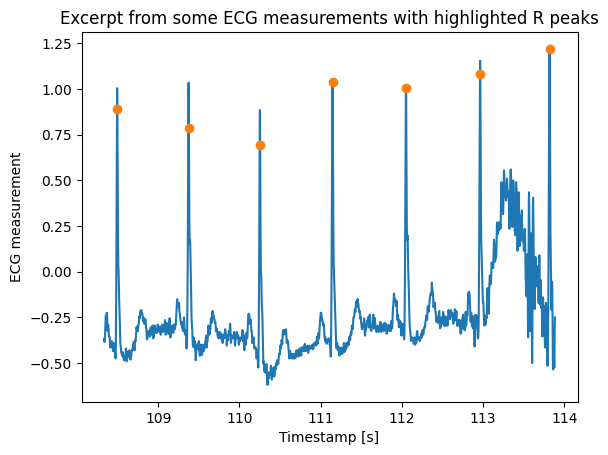
\includegraphics[scale=0.7]{excerpt_ecg_rpeaks.png}
    \caption{Excerpt from one ECG data sample, where the R peaks are highlighted}
\end{figure}

One single, regular heartbeat consists of one so-called QRS complex that consists of three blocks: a Q wave, R wave and S wave. Heartbeat arrhythmia is a medical condition in which the patient experiences an abnormal rhythm of heartbeat. In most cases, this can be diagnosed by looking at the ECG: abnormal shapes in the different blocks or duration can indicate arrhythmia. This can be treated as an anomaly detection problem, where we train a model to learn the probability distribution of regular heartbeats (e.g. to capture their shape characteristics in terms of the building blocks). Based on some decision rule the model can detect samples that come from this distribution or were sampled from a different distribution.

\begin{figure}[h]
    \centering
    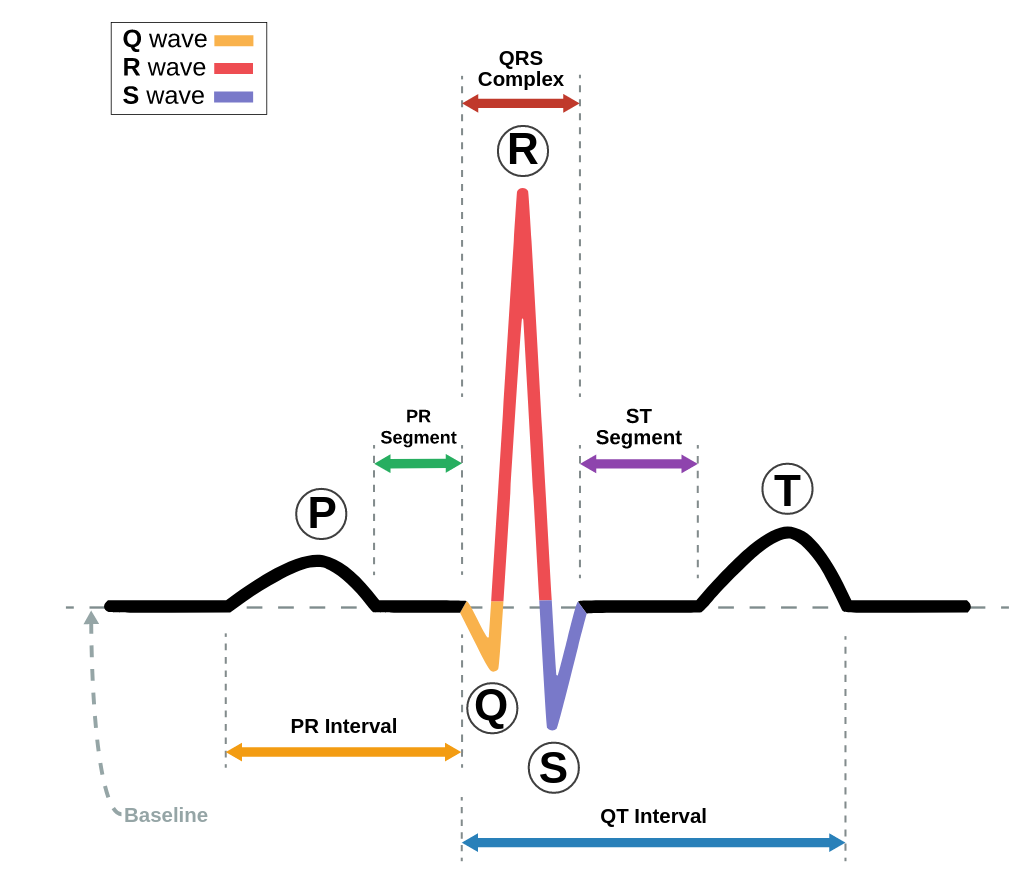
\includegraphics[scale=0.3]{SinusRhythmLabels.png}
    \caption{Schematic represetation of a regular ECG wave, taken from \href{https://en.wikipedia.org/wiki/QRS_complex}{Wikipedia}}
\end{figure}


\begin{figure}[h]
    \centering
    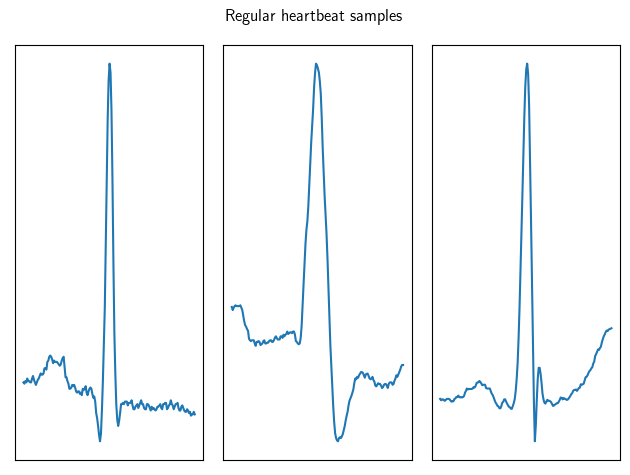
\includegraphics[scale=0.5]{reg_hb_samples.png}
    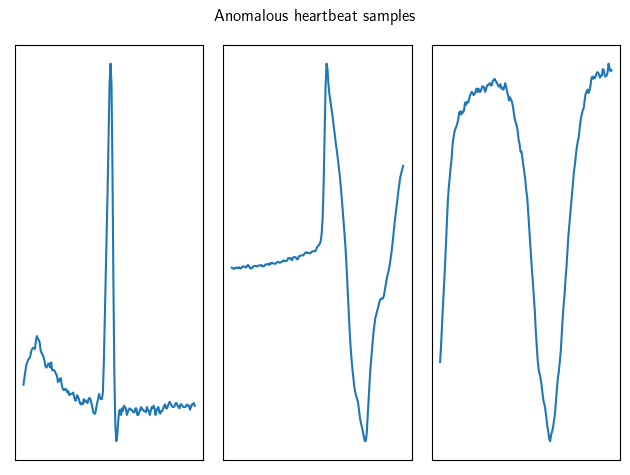
\includegraphics[scale=0.5]{anom_hb_samples.png}
    \caption{Regular and anomalous heart beat samples}
\end{figure}

Before we proceed with the training, we need to preprocess the data. Firstly, since the information contained in both channels are identical, one channel is discarded. We are roughly following the steps from \parencite{ROY2023106484}, where the authors have used an LSTM-autoencoder architecture for arrhythmia detection. This involves normalising the data and extracting single heartbeats from the sequence. To this end, we employ the QRS detector that can detect the R peaks. This is already implemented in the \texttt{wfdb} \parencite{wfdb} package for \texttt{python}. Then, from every peak we consider 90 time steps before and after that peak. This gives one heartbeat with sequence length 180. The associated beat type can then be extracted from the labelled data set. In total this gives over 100 000 single heartbeats each of length 180. We will refer to those samples as private data samples, of which we aim to protect the privacy. In contrast, the generated synthetic data samples will be called public data samples, that we can publish for public use with some associated privacy measure (the privacy is measured by the privacy budget given by the \(\epsilon\) parameter from \cref{def:dp}).

To ensure consistency of results and subsequent comparison of the different model, we split the original data into:
\begin{itemize}
    \item a private training set that consists only of regular samples
    \item a private validation set that consists of roughly equal parts regular and anomalous samples
    \item a private test set that consists of roughly equal parts regular and anomalous samples
\end{itemize}

Therefore, we use the proportions in \cref{fig:tree_test-trainval}.

\begin{figure}[H] \label{fig:tree_test-trainval}
    \centering
    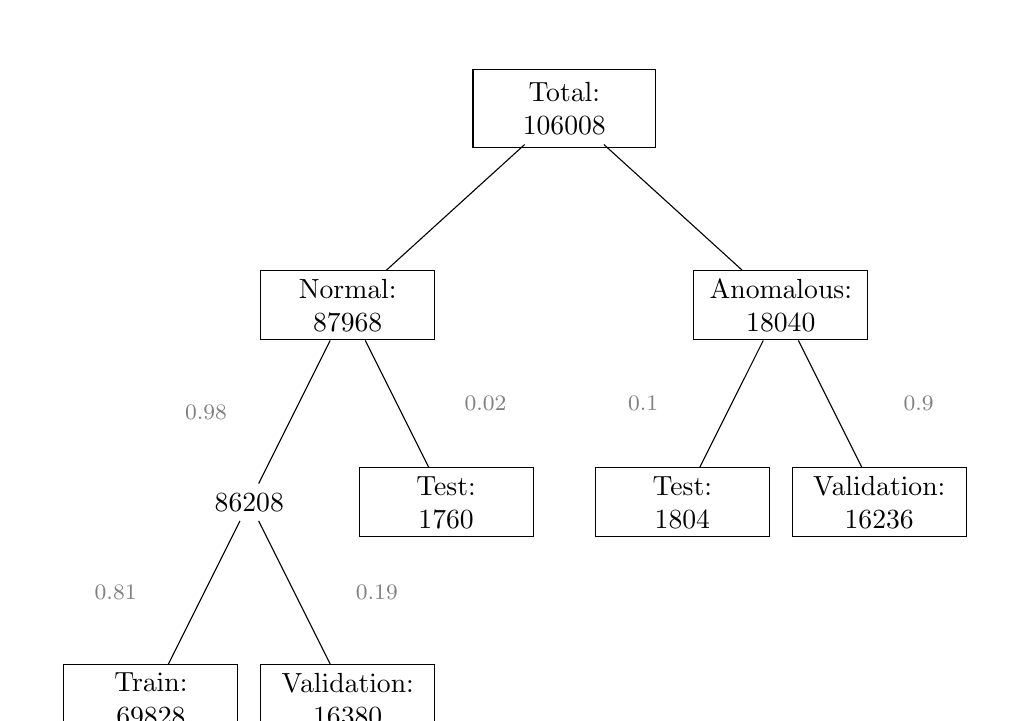
\begin{tikzpicture}[
        level 1/.style={sibling distance=5.5cm},
        level 2/.style={sibling distance=2.5cm},
        edge from parent/.style={draw, -, font=\footnotesize, text=gray}, % Adjust font size and color here
        level distance=2.5cm,
        every node/.style={text width=2cm, align=center}, % Add this line for text width and alignment
        boxed/.style={draw, inner sep=3pt}, % Add this style for the box
    ]
    \node (total) {Total: 106008}
      child {node[boxed] {Normal: \\ 87968}
        child {node {86208}
          child {node[boxed] {Train: \\ 69828} edge from parent node[left] {0.81}}
          child {node[boxed] {Validation: \\ 16380} edge from parent node[right, outer sep=-2pt] {0.19}} % Adjust outer sep
          edge from parent node[left] {0.98}
        }
        child {node[boxed] {Test: \\ 1760} edge from parent node[right] {0.02}}
      }
      child {node[boxed] {Anomalous: \\ 18040}
        child {node[boxed] {Test: \\ 1804} edge from parent node[left] {0.1}}
        child {node[boxed] {Validation: \\ 16236} edge from parent node[right] {0.9}}
      };
    
    % Add a rectangular box around the "Total" node and the "Anomalous" node
    \node[fit=(total), draw, inner sep=1pt] {};
    \end{tikzpicture}
    \caption{Division of the private data set into training, test and validation set}
\end{figure}


All preprocessing tasks and subsequent models are implemented in \texttt{Python 3.7} on a machine running Arch Linux with kernel version 6.7.4 with 16 GB of RAM, an Nvidia RTX 3070 8GB, and AMD 7700 processor with 8 cores / 16 threads. All the code related to this project can be found on on github \footnote{see \href{https://github.com/sjjtu/MAthesis}{https://github.com/sjjtu/MAthesis}}.

\subsection{Baseline Model}
We will establish a baseline model for arrhythmia detection based on an anomaly detection approach from machine learning. One could treat this also as a binary classification problem, but due to the class imbalancy, this would decrease the performance. Hence we are following another idea: one popular solution is to train an autoencoder model on only the regular heartbeats. This way, the model is able to compress regular heartbeat sequence into a latent space and recover them with low reconstruction error. When seeing an anomalous sample, the model fails at properly reconstructing the sample, resulting in a high reconstruction error. We will adjust this error threshold using the validation set, that consists of roughly equal numbers of regular and anomalous samples.

The baseline model is an LSTM-autoencoder with two components, namely:
\begin{itemize}
    \item \underline{Encoder component:} The encoder takes in the one-dimensional heartbeat sequence. There are two LSTM layers that encode the sequence into a latent space. We fixed the dimension of the latent space to 32.
    \item \underline{Decoder component:} The decoder works similar to the encoder but the other way around. Hence, we design it to take in an encoded vector representation of the heartbeat sequence in the latent space with dimension 32 and output a heartbeat sequence one time step after the other.
\end{itemize}

\begin{figure}[h]
    \centering
    \resizebox{0.5\textwidth}{!}{%
    \begin{circuitikz}
    \tikzstyle{every node}=[font=\Large]
    \draw [](6.25,15.5) to[short] (17.5,15.5);
    \draw (6.25,15.5) to[short] (17.5,15.5);
    \draw [](7.5,10.5) to[short] (16.25,10.5);
    \draw [short] (6.25,15.5) -- (7.5,10.5);
    \draw [short] (16.25,10.5) -- (17.5,15.5);
    \draw [](6.25,-2) to[short] (17.5,-2);
    \draw (6.25,15.5) to[short] (17.5,15.5);
    \draw [](7.5,3) to[short] (16.25,3);
    \draw [short] (16.25,3) -- (17.5,-2);
    \draw [short] (6.25,-2) -- (7.5,3);
    \node [font=\LARGE] at (8,15) {Encoder};
    \node [font=\LARGE] at (14.5,2.25) {Decoder};
    \draw [ color={rgb,255:red,94; green,92; blue,100} , dashed] (12,18.25) ellipse (7.75cm and 1cm);
    \node [font=\large] at (11.75,18.25) {Original heartbeats};
    \draw [->, >=Stealth] (12,17) .. controls (12,16.75) and (12,16.5) .. (12,15.75) ;
    \draw [ color={rgb,255:red,94; green,92; blue,100} , dashed] (11.75,-4.75) ellipse (7.75cm and 1cm);
    \node [font=\large] at (11.5,-4.75) {Generated heartbeats};
    \draw [->, >=Stealth] (11.5,-8.5) .. controls (11.5,-9) and (11.5,-9) .. (11.5,-9.75) ;
    \draw  (4,6.75) circle (0.75cm) node {\LARGE $l_1$} ;
    \draw  (6.25,6.75) circle (0.75cm) node {\LARGE $l_2$} ;
    \draw  (8.5,6.75) circle (0.75cm) node {\LARGE $l_3$} ;
    \node [font=\huge] at (13.25,7) {. . . . . . . . . . . . . . . . . . };
    \draw  (17.5,6.75) circle (0.75cm) node {\LARGE $l_{d-1}$} ;
    \draw  (20,6.75) circle (0.75cm) node {\LARGE $l_d$} ;
    \draw  (8.75,13.75) circle (0.5cm) node {\LARGE $s_1$} ;
    \draw  (8,12.75) rectangle  node {\normalsize LSTM} (9.75,11.5);
    \draw  (10.75,12.75) rectangle  node {\normalsize LSTM} (12.5,11.5);
    \draw  (11.5,13.75) circle (0.5cm) node {\LARGE $s_2$} ;
    \draw  (14.5,12.75) rectangle  node {\normalsize LSTM} (16.25,11.5);
    \draw  (15.25,13.75) circle (0.5cm) node {\LARGE $s_n$} ;
    \node [font=\huge] at (13.75,12.25) {. . . };
    \draw [->, >=Stealth] (9.75,12) -- (10.75,12);
    \draw [->, >=Stealth] (15.5,11.5) -- (15.5,8.5);
    \draw [->, >=Stealth] (8.5,5.5) -- (8.5,1.25);
    \draw  (7.75,-0.25) rectangle  node {\normalsize LSTM} (9.5,-1.5);
    \draw  (8.5,0.75) circle (0.5cm) node {\LARGE $l_1$} ;
    \draw [->, >=Stealth] (9.5,-1) -- (10.5,-1);
    \draw  (10.5,-0.25) rectangle  node {\normalsize LSTM} (12.25,-1.5);
    \draw  (11.25,0.75) circle (0.5cm) node {\LARGE $l_2$} ;
    \node [font=\huge] at (13.5,-0.75) {. . . };
    \draw  (14.25,-0.25) rectangle  node {\normalsize LSTM} (16,-1.5);
    \draw  (15,0.75) circle (0.5cm) node {\LARGE $l_d$} ;
    \draw [->, >=Stealth] (15.25,-1.5) -- (15.25,-4.5);
    \draw [->, >=Stealth, dashed] (12.25,-1) -- (14.25,-1);
    \draw [->, >=Stealth, dashed] (12.5,12) -- (14.5,12);
    \draw [->, >=Stealth] (8.75,13.25) -- (8.75,12.75);
    \draw [->, >=Stealth] (8.5,0.25) -- (8.5,-0.25);
    \draw [->, >=Stealth] (11.25,0.25) -- (11.25,-0.25);
    \draw [->, >=Stealth] (15,0.25) -- (15,-0.25);
    \draw [->, >=Stealth] (11.5,13.25) -- (11.5,12.75);
    \draw [->, >=Stealth] (15.25,13.25) -- (15.25,12.75);
    \draw [, dashed] (2.25,9.25) rectangle  (21.25,4.25);
    \node [font=\Large] at (4,8.75) {Latent space};
    \end{circuitikz}
    }%
    
    \label{fig:my_label}
    \caption{Architecture of baseline model}
    \end{figure}

\subsubsection*{Training the Baseline Model}
We train the model on the training set which consists of roughly 70 000 regular heartbeat samples. As loss function we take the mean-squared-error (MSE) between original and reconstructed sample. Training is done using the Adam optimiser with learning rate 5e-4, $\beta_1=0.9$ and $\beta_2=0.999$ for 20 epochs with batch size 1. As we can see from \cref{fig:loss_baseline}, the loss function converges well, indicating a (locally) optimal solution with an average reconstruction error slightly below 1. The loss for the validation set decreases similarly with the training error. This indicates that the model can generalise well to unseen regular heartbeat data.

\begin{figure}[h]
    \centering
    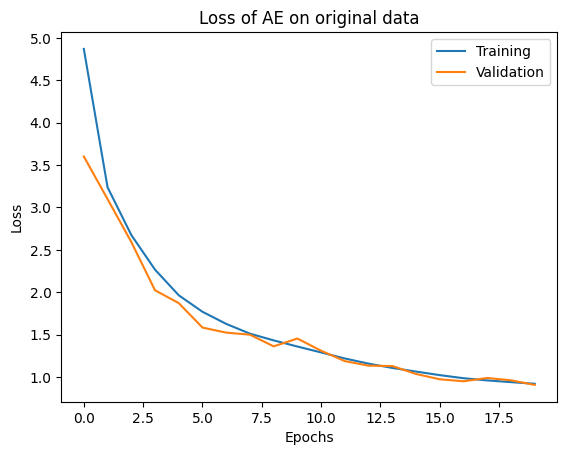
\includegraphics[scale=0.7]{loss_baseline.png}
    \caption{Loss over epoch for baseline model together with loss on validation set}
    \label{fig:loss_baseline}
\end{figure}

With a regular test sample, the model seems to capture all the visually important features and it even removes some of the underlying noise.

\begin{figure}[H]
    \centering
    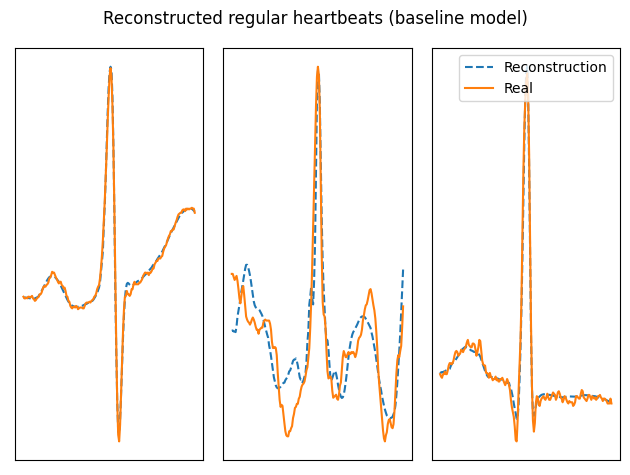
\includegraphics[scale=0.7]{rec_reguarl_samples_baseline.png}
    \caption{Regular test sample vs. reconstructed sample}
    \label{fig:regog_vs_recon}
\end{figure}

Now we do the same but with an anomalous sample for demonstration purposes as can be seen in \cref{fig:anomog_vs_recon}.

\begin{figure}[h]
    \centering
    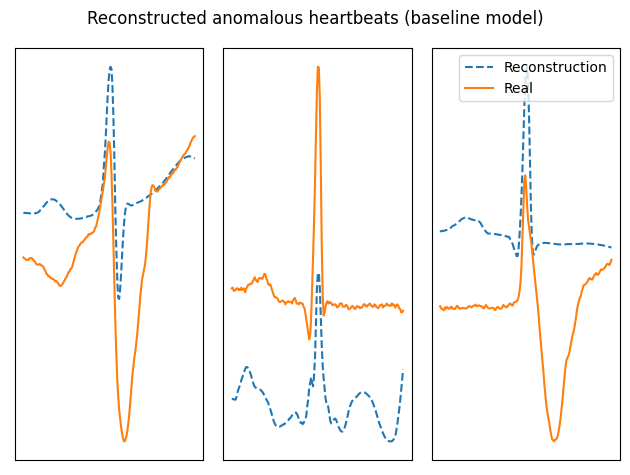
\includegraphics[scale=0.7]{rec_anom_samples_baseline.png}
    \caption{Anomalous test sample vs. reconstructed sample}
    \label{fig:anomog_vs_recon}
\end{figure}

\subsubsection*{Performance of Baseline Model}
So visually, we can already verify that the baseline model seems to be able to distinguish between regular and anomalous samples. We now find an optimal threshold for the reconstruction error and measure the performance. Using the determined theshold value, we do the classification as follows: we input a sample to the anomaly detection model, which outputs the reconstructed sample with some error. If the error is below the threshold, it will be classified as a regular heartbeat, otherwise it will be classified as an anomalous heartbeat. Firstly, let us plot the error distribution on the validation set:

\begin{figure}[H]
    \centering
    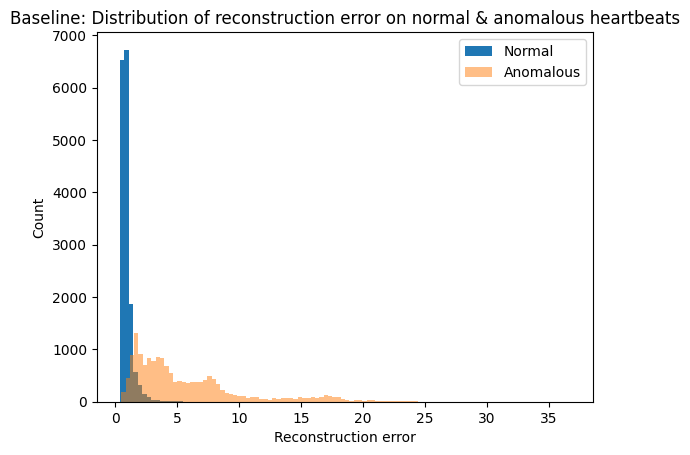
\includegraphics[scale=0.7]{hist_threshold_baseline.png}
    \caption{Distribution of reconstruction error for regular and anomalous samples in the validation set.}\label{fig:distr_err_baseline}
\end{figure}
Clearly, the average error is much lower for regular heartbeats. Thus, the model is able to distinguish regular from anomalous samples by reconstruction error. We can find the ``good'' threshold for the error by computing the percentage of correctly classified regular samples and correctly classified anomalous samples based on different threshold values. In \cref{fig:thres_baseline} we can see that the percentage of correctly classified regular samples slowly increases, while the percentage of correctly classfied anomalous samples decreases. This is to be expected, since a threshold value of 0 would simply classify all samples as anomalous, giving perfect classification for anomalous samples. Conversely, a very high threshold value (e.g. 20) would tend to classify each samples as regular, yielding perfect classification for regular samples. We need to strike a balance between those two extremes by examining \cref{fig:thres_baseline}.

\begin{figure}[h]
    \centering
    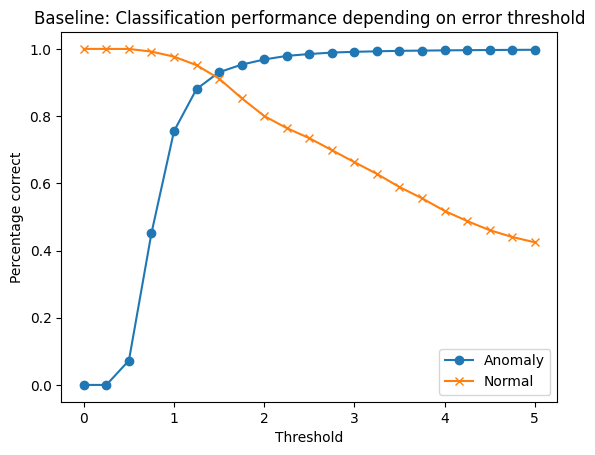
\includegraphics[scale=0.7]{thres_plot_baseline.png}
    \caption{Percentages of correctly classified samples based on different threshold values}
    \label{fig:thres_baseline}
\end{figure}

There are different ways to find a well-suited threshold depending on whether one want to have better performance on anomalous or regular samples. We choose to not favour any classification over the other, hence the neutral decision strategy for the threshold value is the one where both lines cross. Choosing the threshold here to be 1.5, we can compute different metrics that measure the performance of the arrhythmia detection (where TN=True Negatives, TP=True Positives, FN=False Negatives, FP=False Positives):

\begin{itemize}
    \item Accuracy measures the overall percentage of correct classifications:
    \begin{align}
        Accuracy = \frac{TP+TN}{TP+FP+TN+FN} \mperiod
    \end{align}
    \item Precision looks only on the samples that are labelled as anomalies and computes the percentages of correctly detected anomalies:
    \begin{align}
        Precision = \frac{TP}{TP+FP} \mperiod
    \end{align}
    \item Recall looks at all true anomalies and computes the percentage of correctly detected anomalies
    \begin{align}
        Recall = \frac{TP}{TP+FN} \mperiod
    \end{align}
    \item F1 computes the an average of Precision and Recall
    \begin{align}
        F1 = \frac{2\cdot Precision\cdot Recall}{Precision + Recall} \mperiod
    \end{align}
\end{itemize}

\subsubsection*{Summary of Performance Evaluation}
Since we will reuse the previous performance evaluation procedure for measuring the utility of the generated data, we quickly summarise the process:
\begin{enumerate} \label{list:anom_eval}
    \item Train an autoencoder on the synthetic training data set consisting of only regular samples. This synthetic training data is generated by our two different models.
    \item Based on the distribution of the reconstruction errors on the private validation set for regular and anomalous samples, we determine a threshold value for classification.
    \item We evaluate the utility of the generated data based on metrics for anomaly detection.
\end{enumerate}

This approach commonly referred to as the ``Train on synthetic, test on real'' (TSTR) paradigm \parencite{esteban2017realvalued} that is being used to measure utility of synthetic data.

\subsection{Data Generation}
Now we use the models presented in \cref{chapter4} to generate some synthetic heartbeat data. We will train the models on the private training data set, that consists only of regular samples. In turn, the models should be able to generate only regular heartbeat samples. Since both models are similar in architecture, the training procedure can be jointly described as follows.
\begin{enumerate}
    \item We train the autoencoder module separately from rather than jointly with the generator. The authors in \parencite{pei2021towards} have found that there is no significant performance improvement when training jointly. This means, the models first learn how to encode the heartbeat time series in a shared latent space and how to decode it back from it. Conveniently, this is exactly the same autoencoder that is being used by the baseline model for arrhythmia detection, so we do not need to train it again.
    \item We train the generator on encoded training data, i.e. we pass the private training data to the encoder which returns an encoded version of that training data in the latent representation. Then the generator trains to generate this latent representation.
    \item After training, the generator generates a synthetic training set with the same number of samples as the private training set.
    \item We evaluate the utility of the synthetic data by measuring its performance on anomaly detection following the procedure described in \cref{list:anom_eval}.
\end{enumerate}

\subsubsection*{AE-MERF}
We train the AE-MERF model with the configuration in \cref{tab:ae_merf_config}.
\begin{table}[H]
    \centering
    \begin{tabular}{|c|c|c|}
        \hline
        \multirow{4}{*}{\textbf{Autoencoder}}& Embedding dimension & 32 \\ 
                                    & Learning rate & 5e-4 \\
                                    & Number of epochs& 20\\
                                    & Batch size & 1\\
        \hline
        \multirow{4}{*}{\textbf{Generator (MERF)}} & Number of random features & 2000 \\
                                        & Learning rate & 1e-3\\
                                        & Number of epochs & 20\\
                                        & Batch Size & 7000 \\
        \hline
    \end{tabular}
    \caption{Configuration for AE-MERF}
    \label{tab:ae_merf_config}
\end{table}
We then let the model generate some training samples, which are depicted in \cref{fig:aemerf_samples}.

\begin{figure}[h]
    \centering
    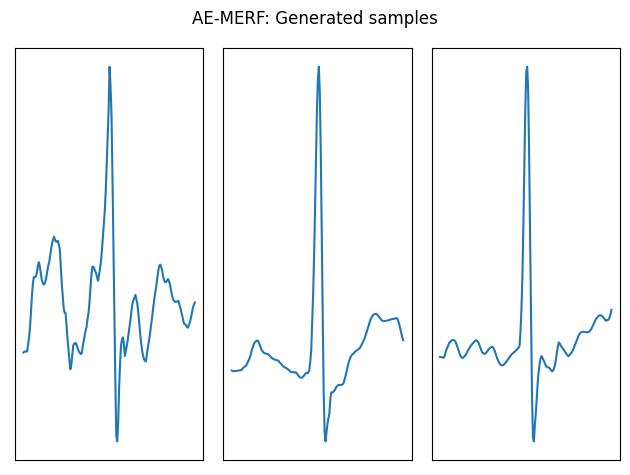
\includegraphics[scale=0.7]{gen_aemerf.png}
    \caption{Generated regular heartbeats by AE-MERF model}
    \label{fig:aemerf_samples}
\end{figure}

To assess the utility, we now train an anomaly detection model with a synthetic training data set. Therefore, we generate a synthetic data set with the same number of samples as the original private training data set, i.e. roughly 70 000 regular heart beat samples. We use the same architecture as for the baseline model - an LSTM autoencoder with embedding dimesion 32. As we can see from the loss in \cref{fig:loss_aemerf}, the model converges on the synthetic training data, while still being able to generalise on the private validation set, that contains real-life samples. The error on the validation set is slightly higher in contrast to the baseline model. The training loss is again slightly below 1 while the validation loss averages around 2. 

\begin{figure}[h]
    \centering
    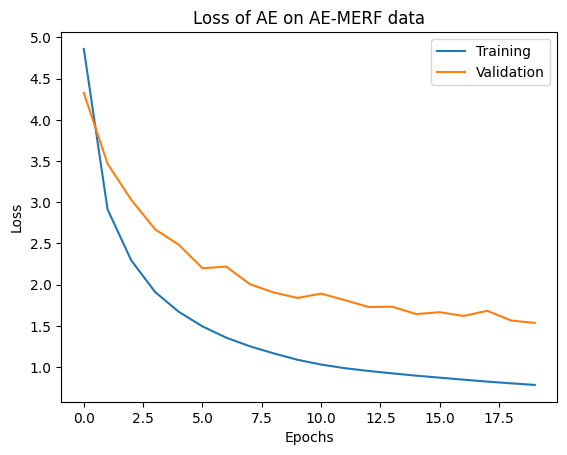
\includegraphics[scale=0.7]{loss_aemerf.png}
    \caption{Loss over epoch for baseline model together with loss on validation set}
    \label{fig:loss_aemerf}
\end{figure}

Now following the established methodology, we compute a good threshold based on which we can distinguish between regular and anomalous samples:

\begin{figure}[h]
    \begin{minipage}[b]{0.45\textwidth}
        \centering
        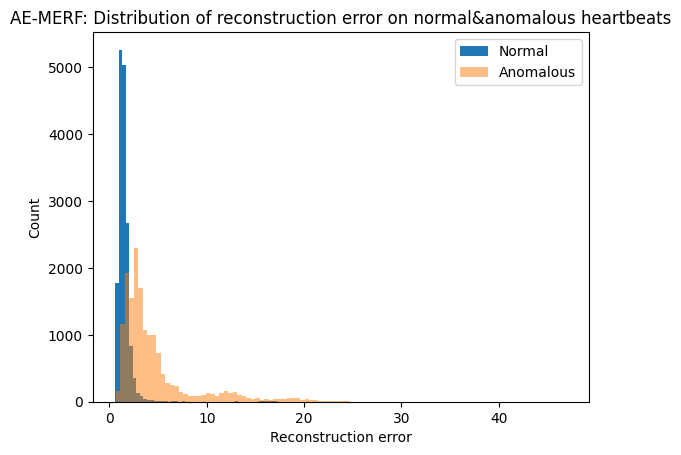
\includegraphics[scale=0.4]{hist_threshold_aemerf.png}
        \caption{Distribution of reconstruction error on validation set with AE-MERF generated samples}
        \label{fig:enter-label}
    \end{minipage}
    \begin{minipage}[b]{0.45\textwidth}
        \centering
        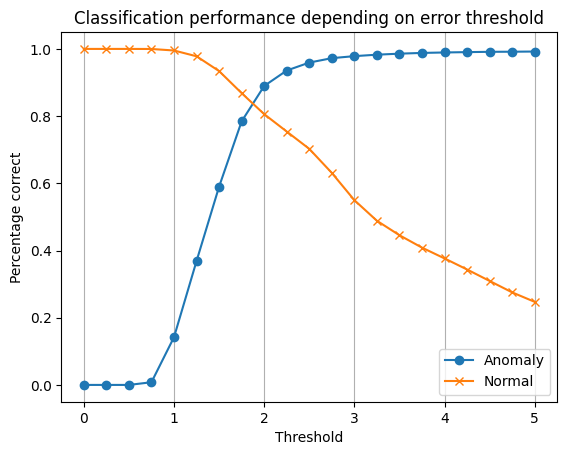
\includegraphics[scale=0.4]{thres_plot_aemerf.png}
        \caption{Percentage of correctly classified regular and anomalous test samples for different threshold values with AE-MERF generated sampled}
        \label{fig:enter-label}
    \end{minipage}
\end{figure}

This gives an error threshold of 1.75. This is slighty higher than threshold computed for the baseline model trained on private data, which indicates that the generator introduced some errors.

\subsubsection*{AE-WGAN}
We train the AE-WGAN model with the configuration in \cref{tab:aewgan_config}.

\begin{table}[h] 
    \centering
    \begin{tabular}{|c|c|c|}
        \hline
        \multirow{4}{*}{\textbf{Autoencoder}}& Embedding dimension & 32 \\ 
                                    & Learning rate & 5e-4 \\
                                    & Number of epochs& 20\\
                                    & Batch size & 1\\
        \hline
        \multirow{4}{*}{\textbf{Generator (WGAN)}} & Discriminator steps & 3 \\
                                        & Learning rate & 9e-3\\
                                        & Number of iterations & 15000\\
                                        & Batch Size & 256 \\
        \hline
    \end{tabular}
    \caption{Configuration for AE-WGAN}
    \label{tab:aewgan_config}
\end{table}

Again, we let the model generate some regular heartbeat samples.
\begin{figure}[H]
    \centering
    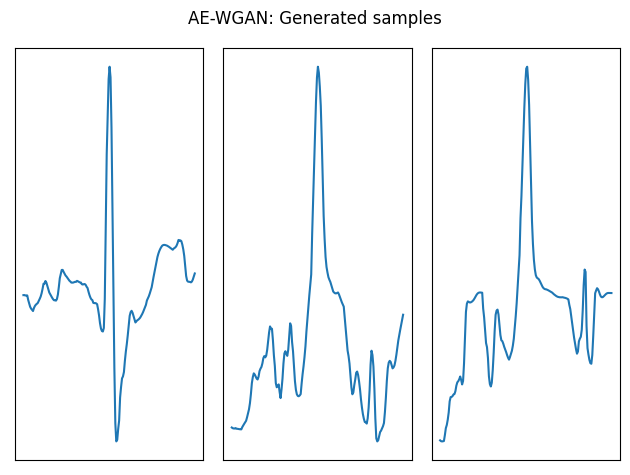
\includegraphics[scale=0.7]{gen_aewgan.png}
    \caption{Generated regular heartbeats by AE-WGAN model}
\end{figure}

Compared to the generated samples from the AE-MERF model, the AE-WGAN model generated samples appear to be much noisier. We expect that the reconstruction error for the arrhythmia detection task will then also be much higher. We again train an LSTM-autoencoder on the synthetic training data generated by AE-WGAN. Looking at the loss, we can see that the validation error is much higher than the training error in this case. This leads to the assumption, that the generated samples differ quite much from the true samples, while still maintaining some important characteristics as the validation is also slowly decreasing.

\begin{figure}[H]
    \centering
    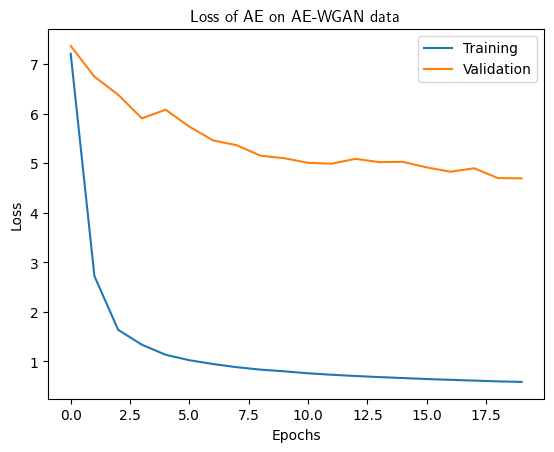
\includegraphics[scale=0.7]{loss_aegwan.png}
    \caption{Loss over epoch for AE-WGAN model together with loss on validation set}
\end{figure}

This behaviour is mirrored when finding the threshold for anomaly detection in \cref{fig:thres_aegwan}
\begin{figure}[h]
    \begin{minipage}[b]{0.45\textwidth}
        \centering
        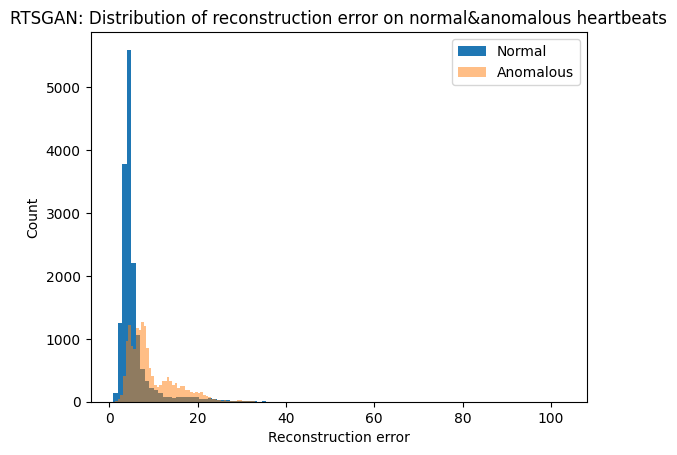
\includegraphics[scale=0.4]{hist_threshold_aewgan.png}
        \caption{Distribution of reconstruction error on validation set with AE-WGAN generated samples}
        \label{fig:enter-label}
    \end{minipage}
    \begin{minipage}[b]{0.45\textwidth}
        \centering
        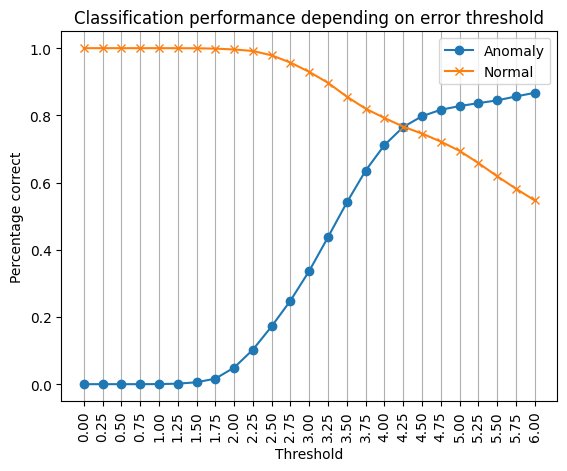
\includegraphics[scale=0.4]{thres_plot_aewgan.png}
        \caption{Percentage of correctly classified regular and anomalous test samples for different threshold values with AE-WGAN generated sampled}
        \label{fig:thres_aegwan}
    \end{minipage}
\end{figure}

The threshold is much higher now, which again confirms the fact, that the samples generated by AE-WGAN deviate much more from the original samples.

\subsection{Privacy-preserving Data Generation}
We now follow the same procedure as previously but add DP noise to each model. How noise is calibrated and added is described in \cref{chapter4}. We follow the same TSTR methodology as for the non-privacy-preserving models. For ease of reading, we omit the plots from training for now and refer to the Appendix if needed. 

\subsubsection*{AE-dpMERF}
We use the DP version AE-dpMERF to generate some samples with DP guarantees. In particular, we generate samples with $\epsilon=1, 0.5, 0.01, 0.001$ and assess their utility for anomaly detection.

\begin{figure}[H]
    \centering
    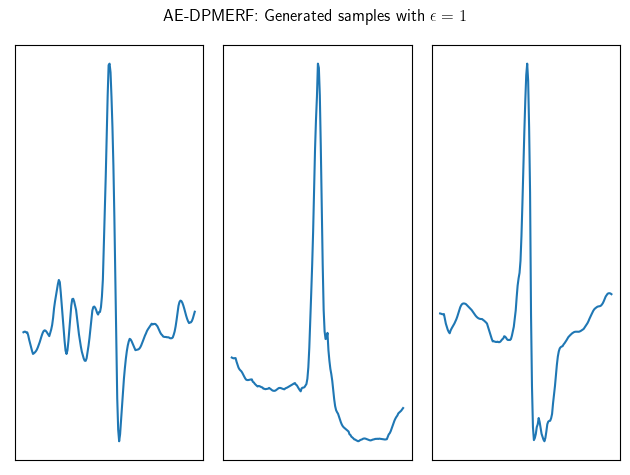
\includegraphics[scale=0.5]{gen_aedpmerf_eps1.png}
    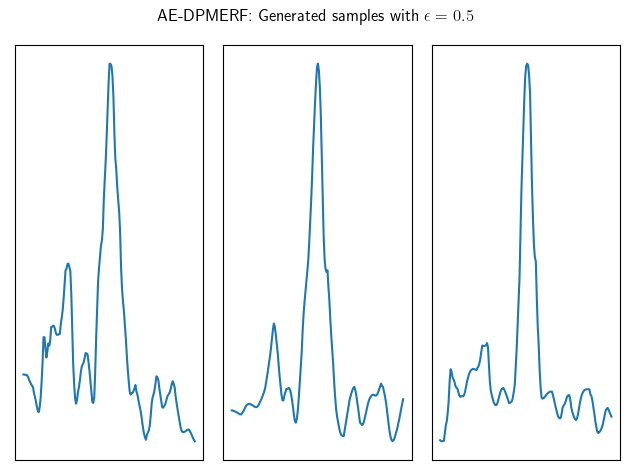
\includegraphics[scale=0.5]{gen_aedpmerf_eps05.png}
    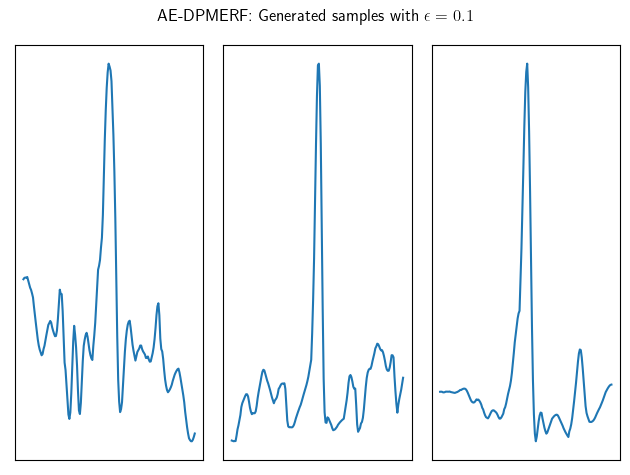
\includegraphics[scale=0.5]{gen_aedpmerf_eps01.png}
    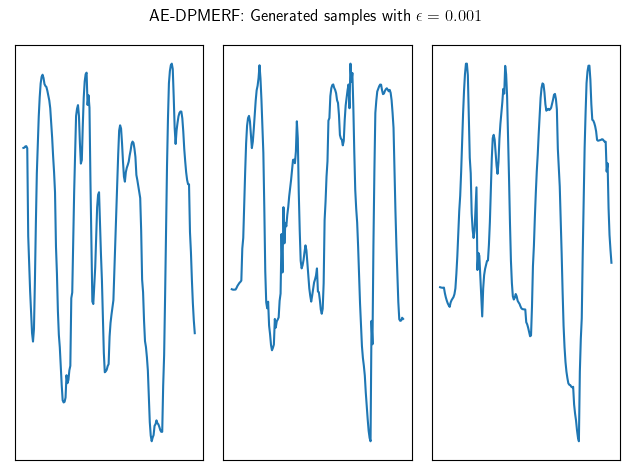
\includegraphics[scale=0.5]{gen_aedpmerf_eps001.png}
    \caption{AE-dpMERF generated samples with different $\epsilon$, the lower the value the higher the privacy guarantees}
    \label{fig:gen_aedpmerf}
\end{figure}

As we can see, the lower the $\epsilon$ privacy parameter the more noise is introduced. This gives stricter privacy guarantees, but for $\epsilon=0.001$ too much noise is added and the generated samples visually do not appear to show a regular heartbeat. Clearly we can see from the generated samples in \cref{fig:gen_aedpmerf}, that more noise during training also results in more noise for the generated samples.  In practice, it is recommended to use an $\epsilon$ value of 1, so AE-dpMERF with $\epsilon=1$ already gives visually satisfying results \parencite{dwork2019differential}.

\subsubsection*{AE-dpWGAN}
We use the DP version AE-dpWGAN to generate some samples with DP guarantees and $\epsilon=35, 25, 5$. As the training for GANs is inherently very unstable and therefore sensitive to changes, we did not obtain satisfying results with even lower epsilon values. 

\begin{figure}[H]
    \centering
    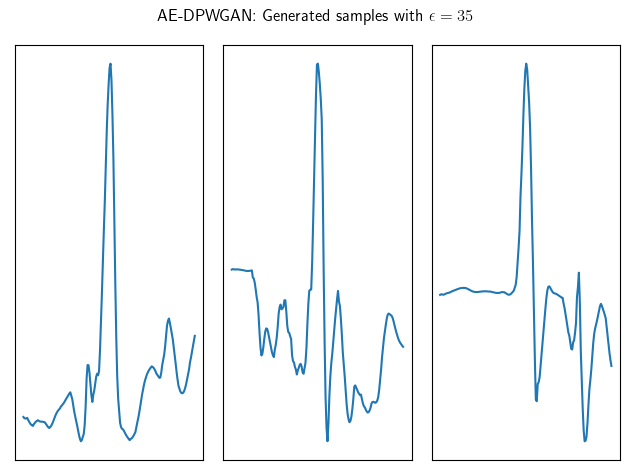
\includegraphics[scale=0.6]{gen_aedpwgan_eps35.png}
    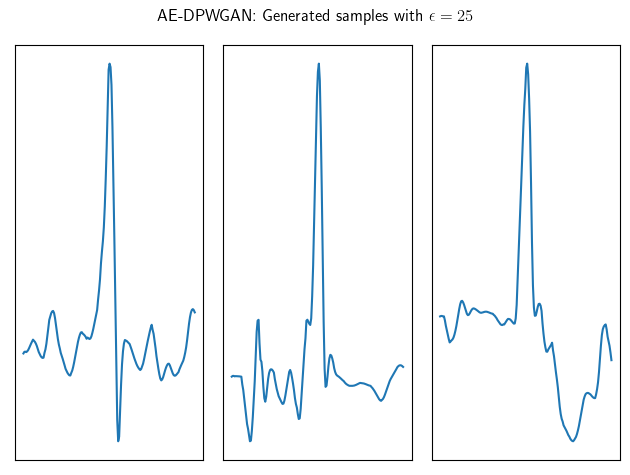
\includegraphics[scale=0.6]{gen_aedpwgan_eps25.png}
    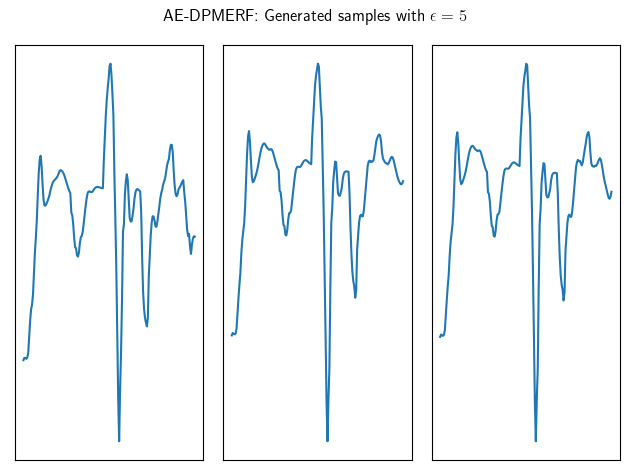
\includegraphics[scale=0.6]{gen_aedpwgan_eps5.png}
    \caption{AE-dpWGAN generated samples with different $\epsilon$, the lower the value the higher the privacy guarantees}
\end{figure}

As we can see, even with $\epsilon=35$ there is a lot of visible noise in the generated samples. This behaviour aggravates with decreasing $\epsilon$. When training with $\epsilon=5$ too much noise is added and the GAN becomes really hard to train properly. 

\subsection{Results}
We are now ready to compare all the different models in terms of their performance on anomaly detection. \cref{tab:results} shows a summary of all models with their performance scores. We also summarise this information in \cref{fig:res_aedpmerf}. It is apparent that utility is lost already during (non-privacy-preserving) data generation. The loss in utility is around 10\% for AE-MERF and 15\% for AE-WGAN. Additionally, surprisingly we see that their is no significant loss in utility when introducing differential privacy to either models up to a certain $\epsilon$ value. For AE-dpMERF with $\epsilon=0.5, 1$ the recall value is even higher than for the baseline model. Of course, the generated samples contain much more noise, thus leading to higher reconstruction error as we have seen before, but this does not impact the anomaly detection performance much. Once the $\epsilon$ value is too low, thus too much noise is added during generation, the generated samples loose their utility for anomaly detection. For AE-dpMERF the lowest observed value is $\epsilon=0.5$ for which we do not see a decrease in utility. On the other, synthetic samples generated by AE-dpWGAN become too noisy already with much higher $\epsilon$ values, e.g. $\epsilon=5$. 
\begin{table}[h]
    \centering
    \begin{tabular}{c||c|c|c|c}
        \textbf{Model} & \textbf{Accuracy} & \textbf{Precision} & \textbf{Recall} & \textbf{F1} \\ 
        \hline 
        \hline

        Baseline & 0.92 & 0.91 & 0.94 & 0.92 \vspace{0.5cm}\\
        \hline

        AE-MERF & 0.83 & 0.85 & 0.79 & 0.82 \\
        \hline
        AE-DPMERF ($\epsilon=1$) & 0.83 & 0.81 & 0.86 & 0.83 \\
        \hline
        AE-DPMERF ($\epsilon=0.5$) & 0.81 & 0.81 & 0.80 & 0.80 \\
        \hline
        AE-DPMERF ($\epsilon=0.1$) & 0.76 & 0.75 & 0.77 & 0.76\\
        \hline
        AE-DPMERF ($\epsilon=0.01$) & 0.48 & 0.47 & 0.41 & 0.43 \vspace{0.5cm}\\
        \hline

        AE-WGAN & 0.76 & 0.75 & 0.75 & 0.75 \\
        \hline
        AE-DPWGAN ($\epsilon=35$) & 0.74 & 0.74 & 0.75 & 0.74 \\
        \hline
        AE-DPWGAN ($\epsilon=25$) & 0.72 & 0.73 & 0.71 & 0.71 \\
        \hline
        AE-DPWGAN ($\epsilon=5$) & 0.56 & 0.56 & 0.57 & 0.56\\

    \end{tabular}
    \caption{Summary of anomaly detection performance}
    \label{tab:results}
\end{table}

\begin{figure}[H]
    \centering
    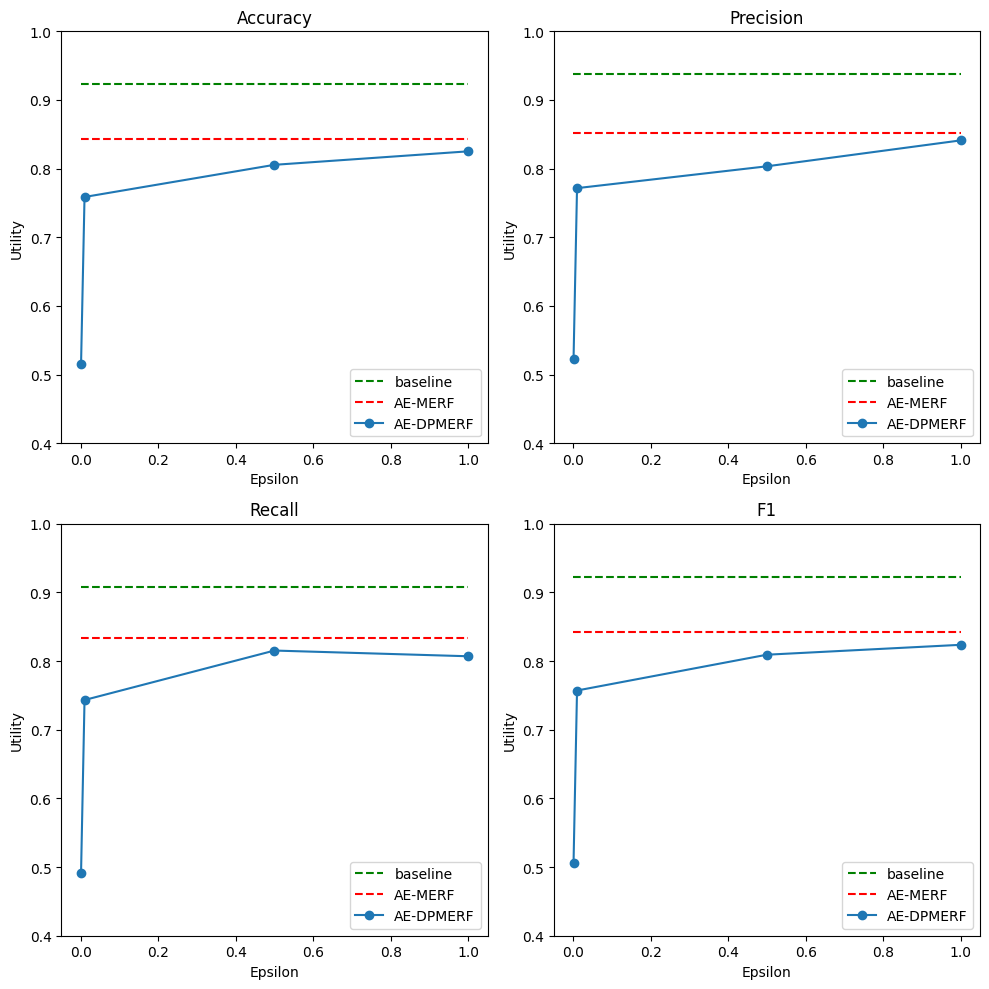
\includegraphics[scale=0.6]{results_aedpmerf.png}
    \caption{Utility loss over privacy budget $\epsilon$ for AE-(dp)MERF}
    \label{fig:res_aedpmerf}
\end{figure}

\begin{figure}[H]
    \centering
    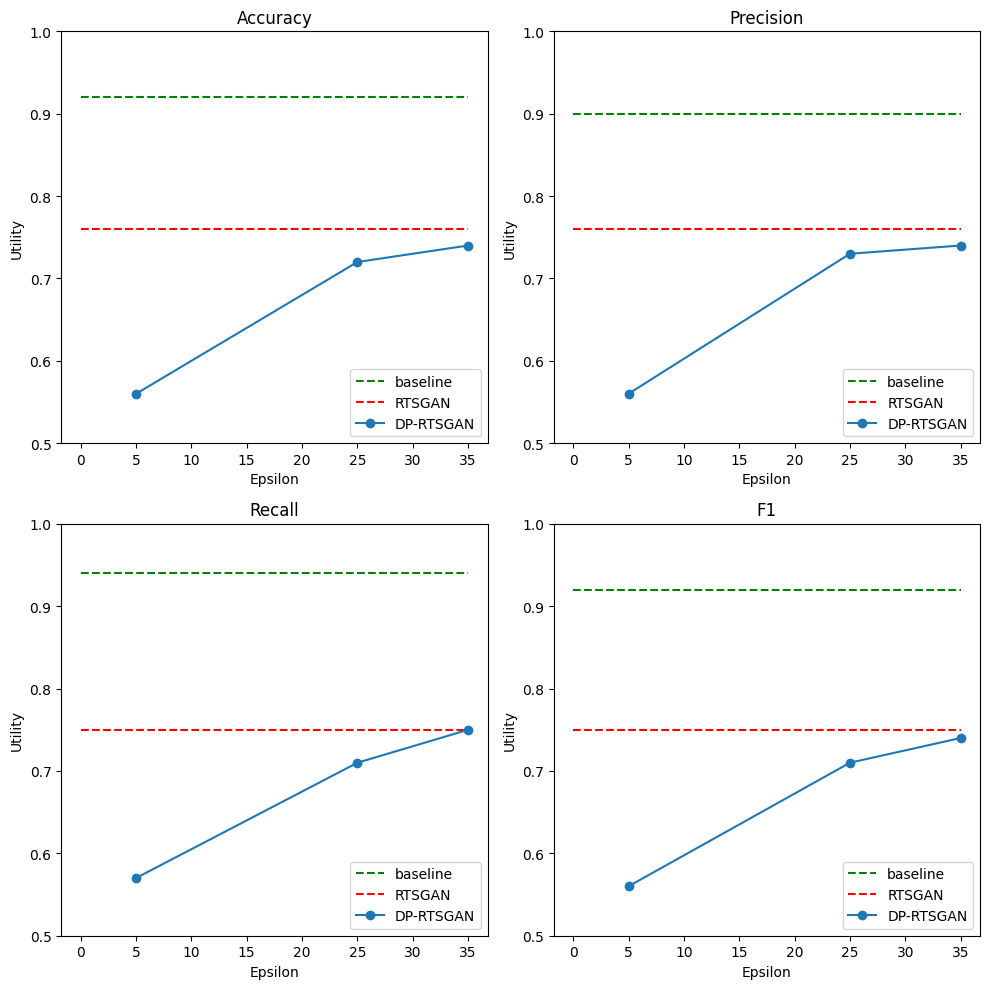
\includegraphics[scale=0.6]{restuls_dprtsgan.png}
    \caption{Utility loss over privacy budget $\epsilon$ for AE-(dp)WGAN}
    \label{fig:res_aedpmerf}
\end{figure}

\subsection{Contaminated Data Set}
Now we contaminate the original training set that previously consisted of regular heartbeat samples only with some anomalous ones. This serves two purposes:
\begin{enumerate}
    \item In real-life, labelled data is rare and heartbeat arrhythmia are scarce (1.5 - 5\%). Having a contaminated training data set can simulate this scenario. Additionally, labelling errors or ambiguous cases can lead to a contaminated data set as well.
    \item We can check how adding DP to the generation procedure will impact the robustness of the generated samples. 
\end{enumerate}

Therefore, we contaminate the training data with 1\%, 2\% and 5\% of anomalous heartbeat samples and repeat the data generation and anomaly detection as before only for the AE-(dp)MERF models with $\epsilon=1, 0.5$ since they delivered promising results.

\begin{figure}[H]
    \centering
    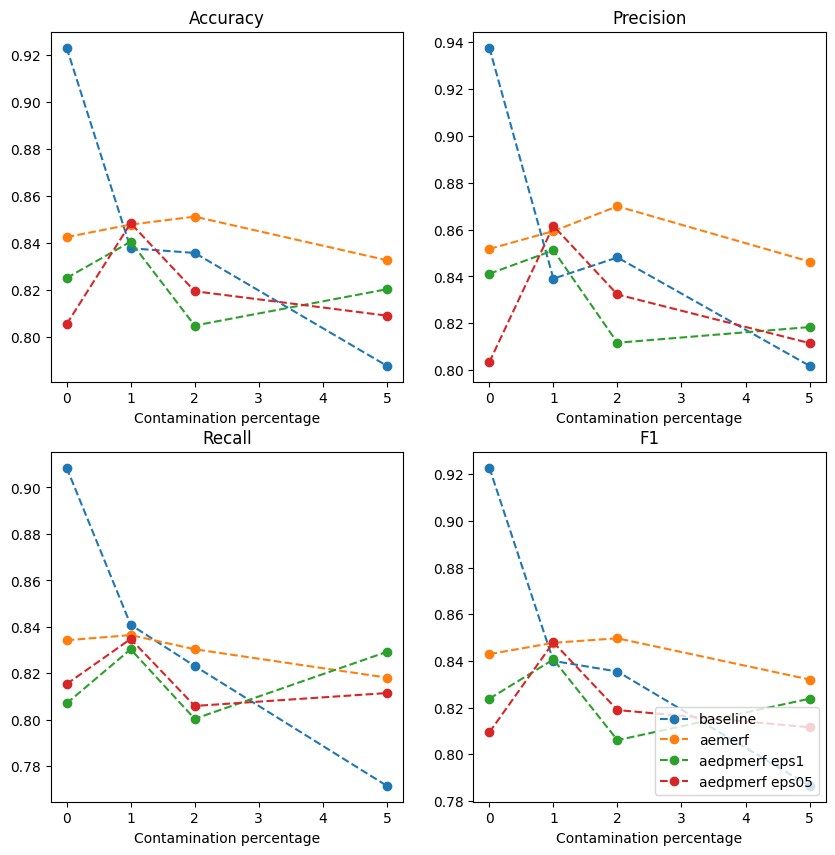
\includegraphics[scale=0.7]{results_aedpmerf_contam.png}
    \caption{AE-(dp)MERF on contaminated training data}
    \label{fig:res_contam_aedpmerf}
\end{figure}

Looking only at the baseline model (blue line in \cref{fig:res_contam_aedpmerf}), we can clearly see that the performance decreases with higher contamination level. There is a slight increase for the precision metric when going from 1\% contamination to 2\%. This is to be expected, since precision measures the correctly detected anomalies among all detected anomalies, i.e. $Precision=\frac{TP}{TP+FP}$. When contaminating the training data set with anomalous samples, the number of undetected anomalies (FN) will increase and thus the number of wrongly detected anomalies (FP) will decrease, which in turn results in a higher precision.

The non-privacy-preserving AE-MERF model behaves similarly, but the impact of the contamination is smaller. This means that using AE-MERF generated samples is more robust than using the original private samples. This robustness transfers to the DP version: For both privacy-preserving models AE-dpMERF the performance metrics initially increase for a contamination level of 1\%, before decreasing, when the contamination increases up to 5\%. Surprisingly, for the highest contamination of 5\%, the anomaly detection model trained with synthetic data outperforms the baseline model. 



	\section{Discussion}

\subsection{(Privacy-Preserving) Data Generation}
From our experiments, we can clearly see that the AE-(dp)MERF generated samples achieved a much higher utility compared to the GAN-based approach. This confirms the result from \parencite{hu2023sok} stating DP-MERF is the ``best all purpose generator''. We found that AE-(dp)MERF also performs well on time series data, which has not been examined prior to this work to the best of our knowledge. Of course, further data and models need to be tested for verification. Adding privacy was straight forward to implement for AE-(dp)MERF and the training of the generator worked well in even lower $\epsilon$ regimes. This is not the case for the GAN-based approache: due to the inherent stability issues with training GANs, adding noise during the process imposes even more instabilities into the training process. Thus, training with even higher \(\epsilon\) values required a careful selection of hyperparameters.


\subsection{Utility-Privacy-Tradeoff}

Many studies suggest, that adding (differential) privacy to a model decreases its utility. Our result suggest, that this tradeoff is more nuanced and depends on the use case and the utility measure. The conducted experiments show, that for reasonable $\epsilon$ values and depending on the generator, utility of synthetic, privacy-preserving data and privacy can go hand in hand. We have observed only a slight decrease in utility when employing DP to our models. For AE-(dp)MERF using $\epsilon=$ values as low as 0.5 did not ``destroy'' utility. The GAN-based model behaved similarly, but with much higher \(\epsilon\) values ($\epsilon=25$). However, this only applies to anomaly detection and does not say something about the quality of the generated samples. On the contrary, we have seen that the generated samples appear much noisier when we add differential privacy to the generation process.

\subsection{Privacy and Robustness}
In the last experiment, we contaminated the private training set with anomalous samples. While the baseline modelled trained directly on this contaminated data set saw a steep decrease in performance, models trained with non-privacy-preserving, synthetic data generated by AE-MERF achieved much more stable results. This could be attributed to how the mean embeddings are computed (see \cref{eq:rff}): We hypothesise, that the inherent randomness from computing the random Fourier features has a regularising effect. This needs to be examined further.

Additionally, the DP generated samples based on contaminated training data not only exhibit the same robustness but even for low contamination levels even improved its utility. A similar result has been observed in \parencite{du2019robust}. A possible explanation lies in the nature of DP: by definition, DP bounds the influence one particular sample can have on the outcome. In particular, this can hide the presence of the small amount of anomalous heartbeat samples that were injected into the training data. This has to be verified rigorously.


\subsection{Future Works}

We have tested two different privacy-preserving algorithms for ECG time series data generation using th MITBIH data set. Although those algorithms fulfill differential privacy. This is a probabilistic framework for assessing privacy and needs to be tested empirically. One could follow the works of \colorbox{red}{ref}. 
Furthermore, as we have only used the models to generated ECG data for arrhythmia detection, our findings need to be confirmed on other common benchmarking data set, e.g. \colorbox{red}{tba.}.
Lastly, our experiments show an useful connection between (differential) privacy and robustness, which opens new lines of research for privacy-preserving and robust data generation algorithms.



	\section{Outro}

\subsection{Future Works}
\begin{itemize}
    \item test attacks to verify empirically
    \item test with other time series data
    \item rigorous hyperparameter tuning
    \item 
\end{itemize}
\subsection{Conclusion}

	\clearpage

	\pagestyle{plain}
	\pagenumbering{Roman}
	\setcounter{page}{1}
	\section*{Appendix}

	\addcontentsline{toc}{section}{Appendix}
	\clearpage

	\printbibliography[heading=bibintoc, title=References]
	\clearpage
\end{document}
